\chapter{Notes on the data in the M6 signal region}
    \label{app:scaleFactorEvolution}

Section~\ref{sec:ResultsSR} shows a two sigma-level discrepancy between the data and the SM prediction in the signal region M6.
In order to study whether this excess is due to a mismodeling in the Standard Model backgrounds, several distributions are studied in the different control regions.
Figure~\ref{fig:Plot_M6_CRwmn_Jetkinematics} shows, in the $\wmn$+jets control region, the module and the azimutal angle $\phi$ of the $\met$, the $\pt$ and the $\eta$ of the leading jet, the $\pt$ of the second leading jet and the ratio between the $\met$ and the leading jet $\pt$.
In Figure~\ref{fig:Plot_M6_CRwmn_Leptonkinematics}, the muon $\pt$, $\eta$, $\phi$ and the transverse mass are shown.
Similar distributions are presented for the $\wen$+jets and $\zmm$+jets control regions in Figures~\ref{fig:Plot_M6_CRele_Jetkinematics} and \ref{fig:Plot_M6_CRele_Leptonkinematics}, \ref{fig:Plot_M6_CRzmm_Jetkinematics} and \ref{fig:Plot_M6_CRzmm_Leptonkinematics}, respectively.

\begin{figure}[!ht]
  \begin{center}
    \mbox{
      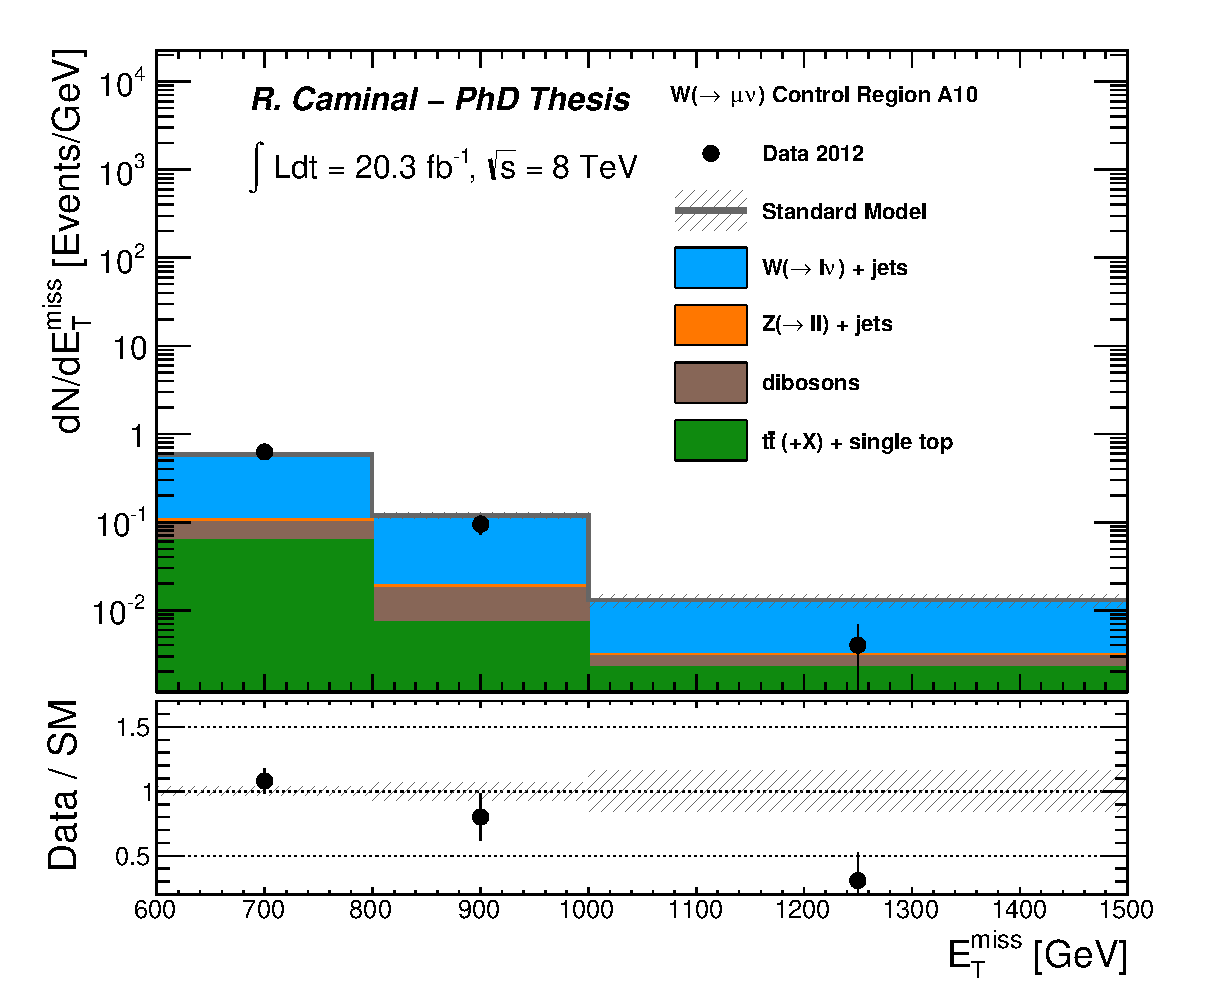
\includegraphics[width=0.495\textwidth]{Appendix_FluctuationM6/Figures/plot_Stop_A10_CRwmn_met_fitted.eps}
      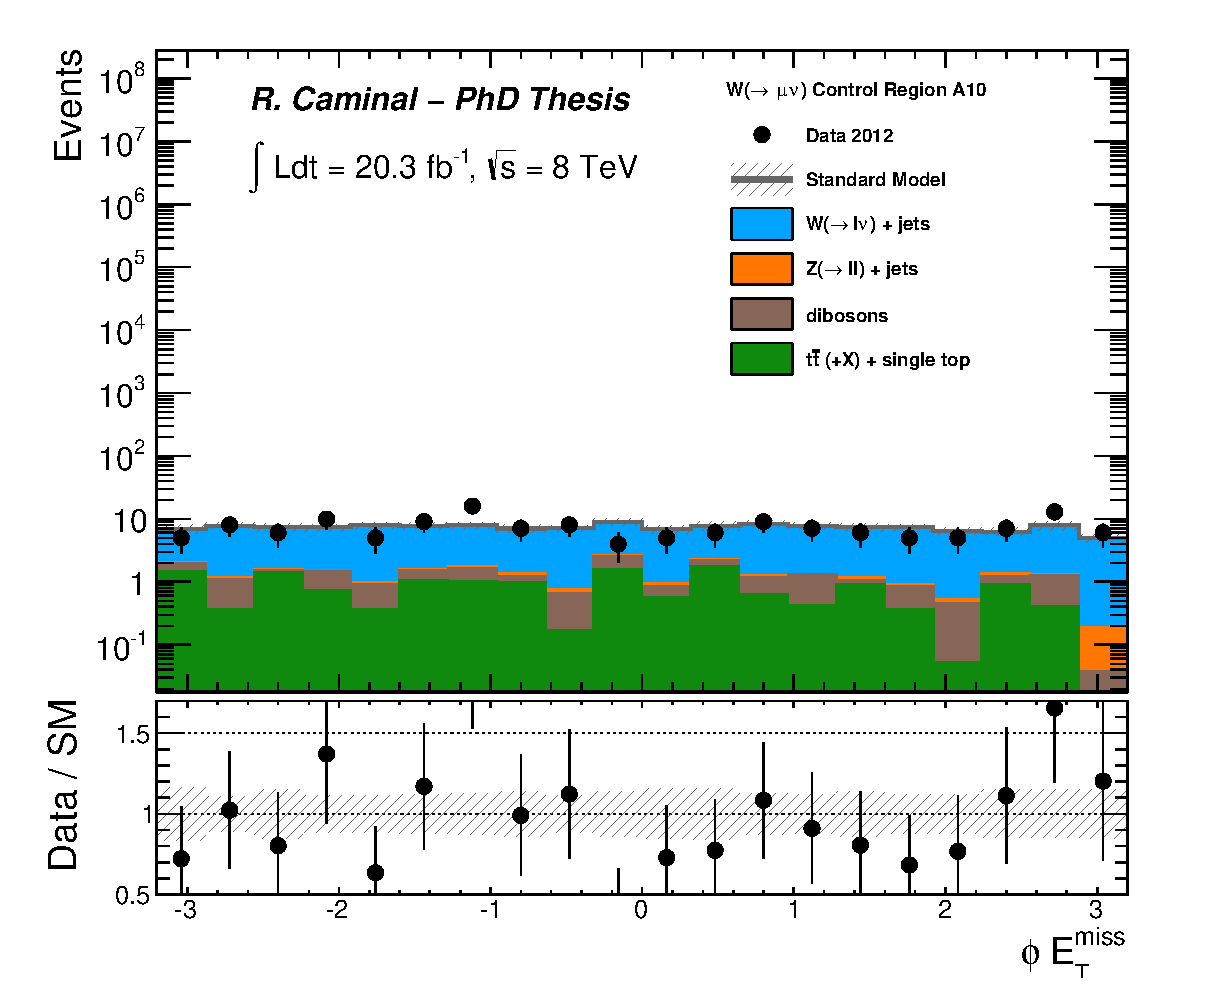
\includegraphics[width=0.495\textwidth]{Appendix_FluctuationM6/Figures/plot_Stop_A10_CRwmn_met_phi_fitted.eps}
    }
    \mbox{
      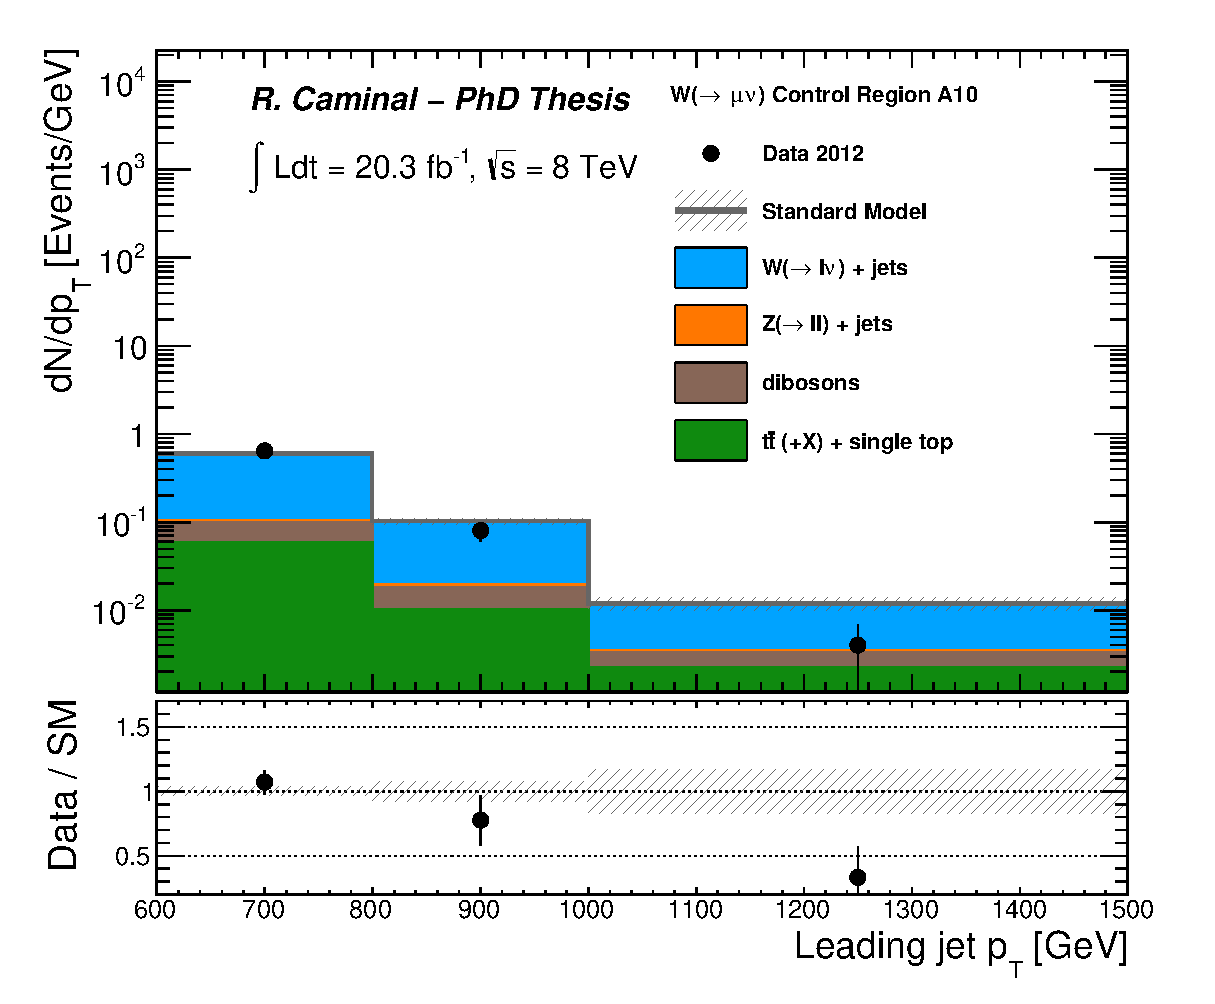
\includegraphics[width=0.495\textwidth]{Appendix_FluctuationM6/Figures/plot_Stop_A10_CRwmn_pt1_fitted.eps}
      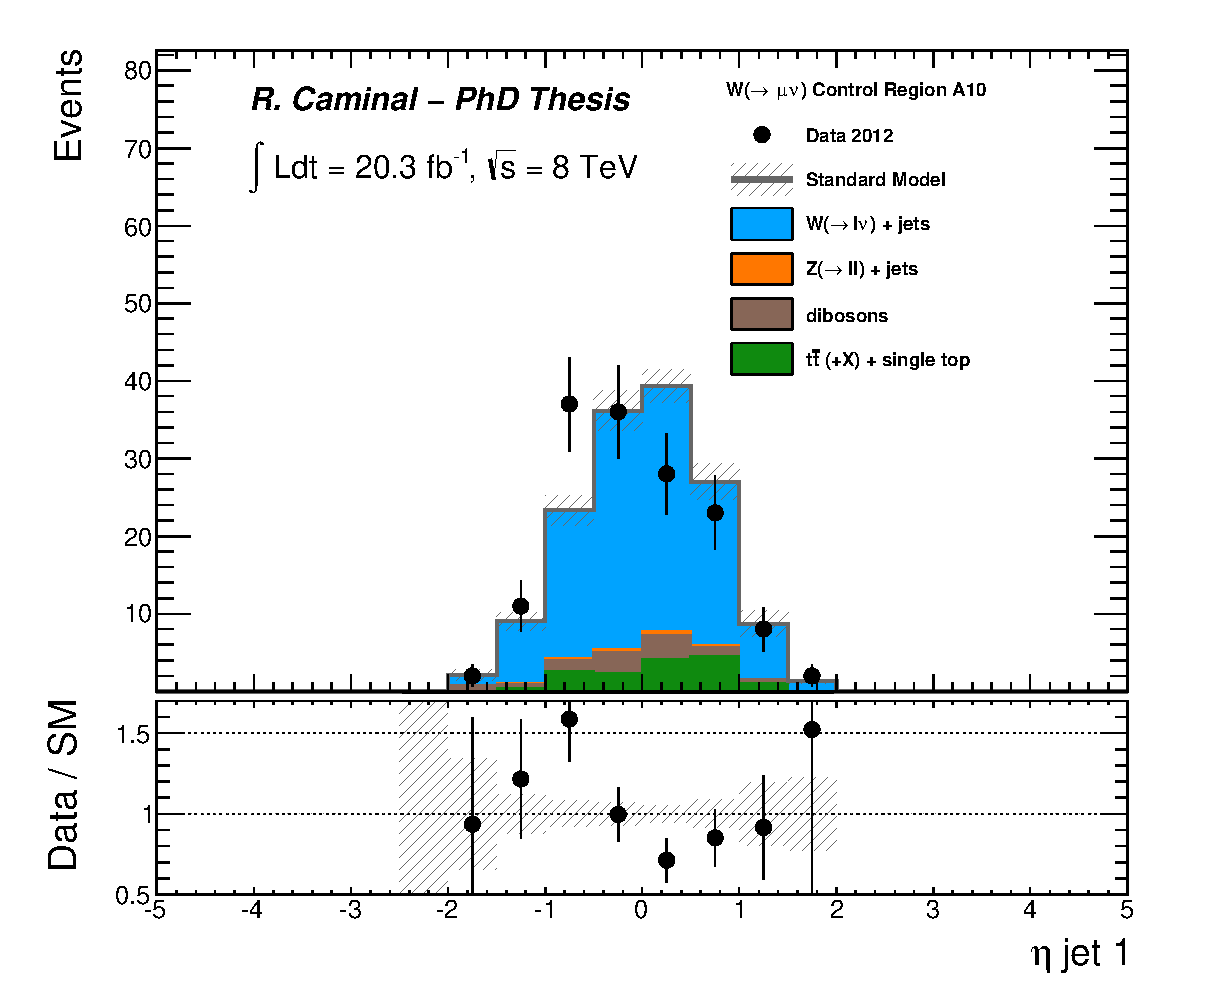
\includegraphics[width=0.495\textwidth]{Appendix_FluctuationM6/Figures/plot_Stop_A10_CRwmn_eta1_fitted.eps}
    }
    \mbox{
      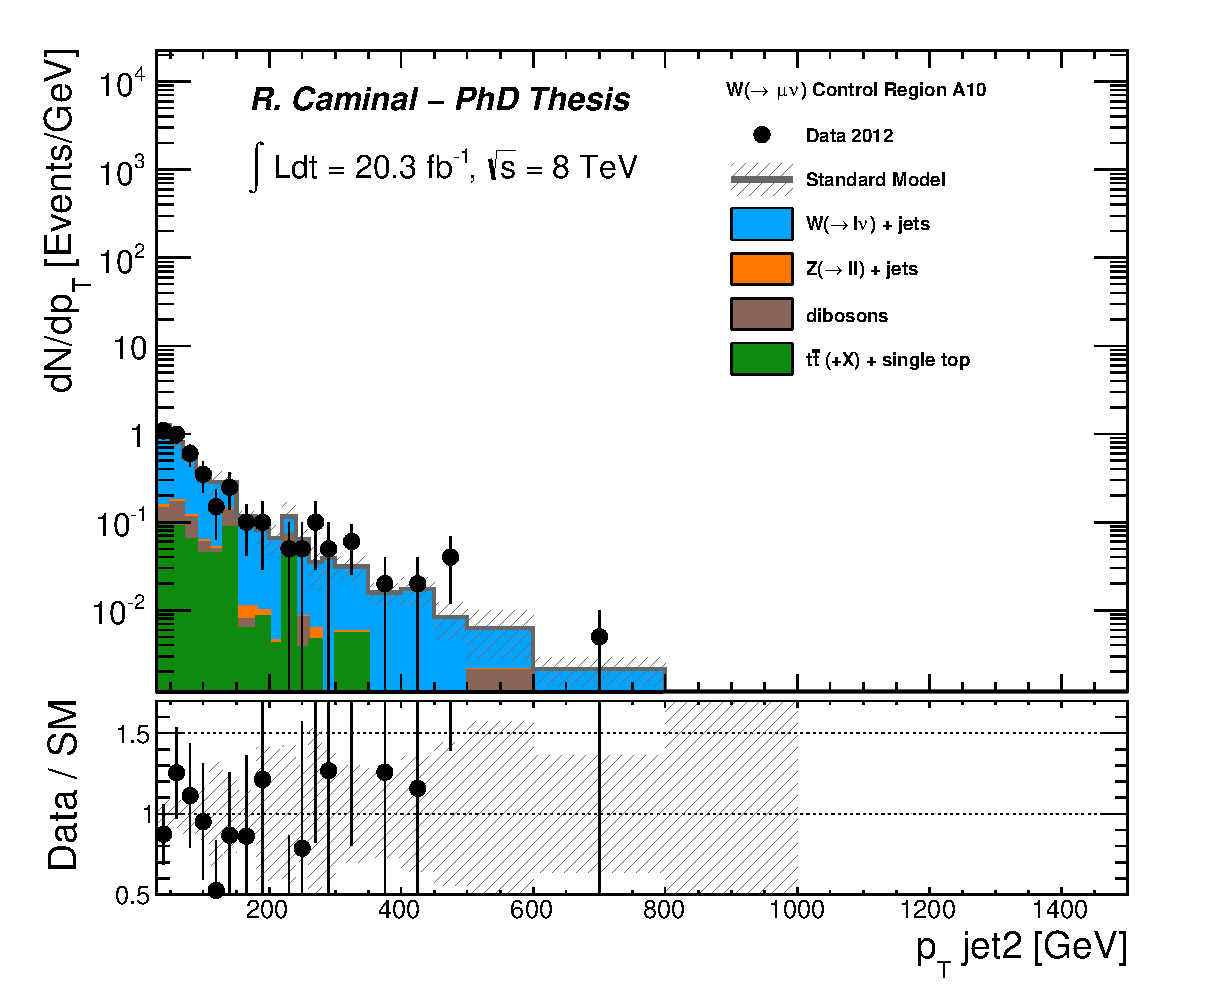
\includegraphics[width=0.495\textwidth]{Appendix_FluctuationM6/Figures/plot_Stop_A10_CRwmn_pt2_fitted.eps}
      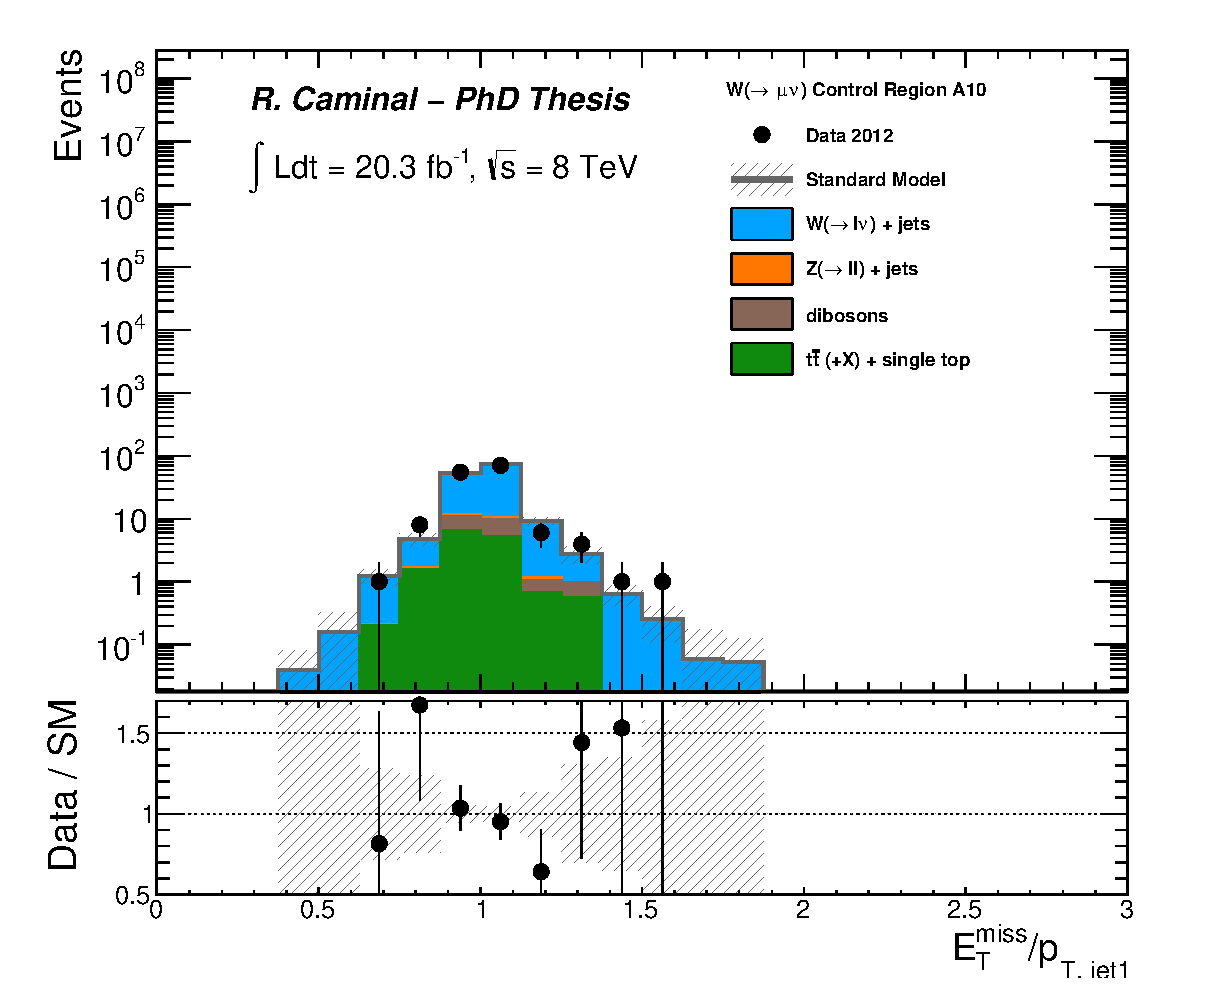
\includegraphics[width=0.495\textwidth]{Appendix_FluctuationM6/Figures/plot_Stop_A10_CRwmn_metpt1_fitted.eps}
    }
  \end{center}
  \caption[Kinematic distributions of the reconstructed jets and $\met$ in the $\wmn$+jets control region for the selection cuts of region M6, after the normalization factors extracted from the fit have been applied.]{The measured kinematic distributions of the reconstructed jets and $\met$ in the $\wmn$ control region for the selection cuts of region M6 compared to the background predictions. The latter include the global normalization factors extracted from the fit. The error bands in the ratios include the statistical and experimental uncertainties on the background predictions.}
  \label{fig:Plot_M6_CRwmn_Jetkinematics}
\end{figure}

\begin{figure}[!ht]
  \begin{center}
    \mbox{
      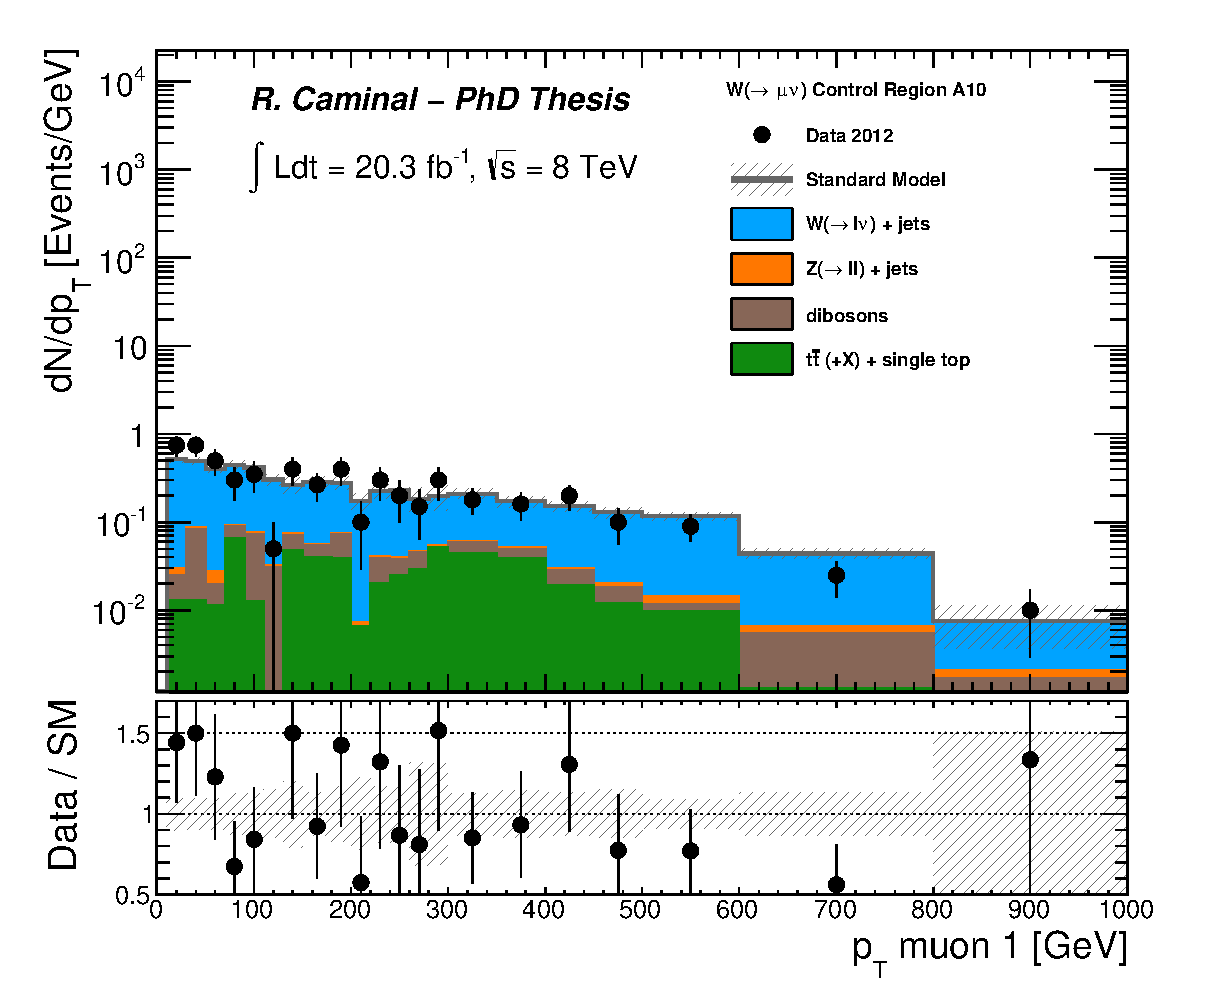
\includegraphics[width=0.495\textwidth]{Appendix_FluctuationM6/Figures/plot_Stop_A10_CRwmn_m_pt_fitted.eps}
      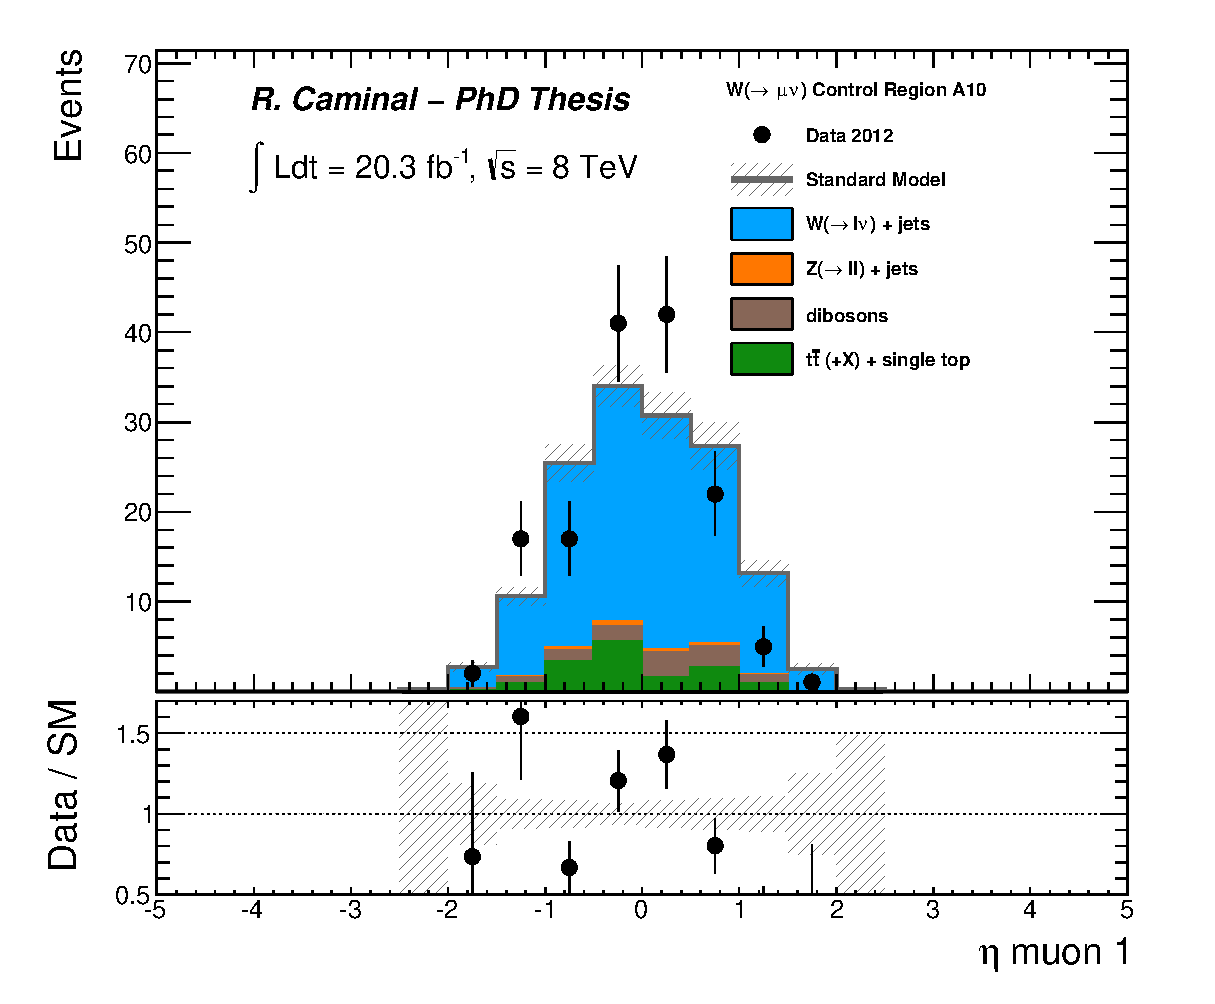
\includegraphics[width=0.495\textwidth]{Appendix_FluctuationM6/Figures/plot_Stop_A10_CRwmn_m_eta_fitted.eps}
    }
    \mbox{
      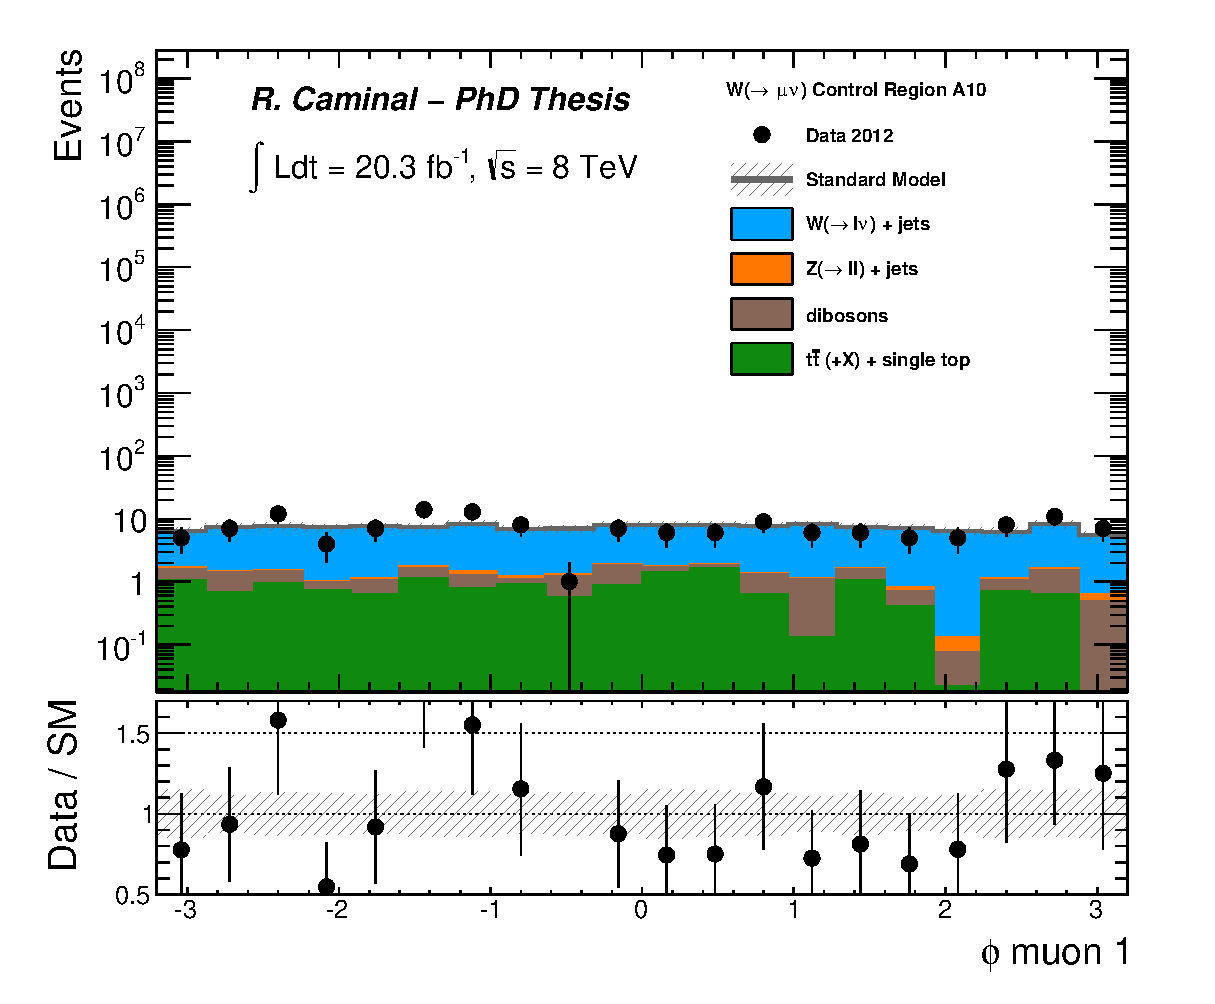
\includegraphics[width=0.495\textwidth]{Appendix_FluctuationM6/Figures/plot_Stop_A10_CRwmn_m_phi_fitted.eps}
      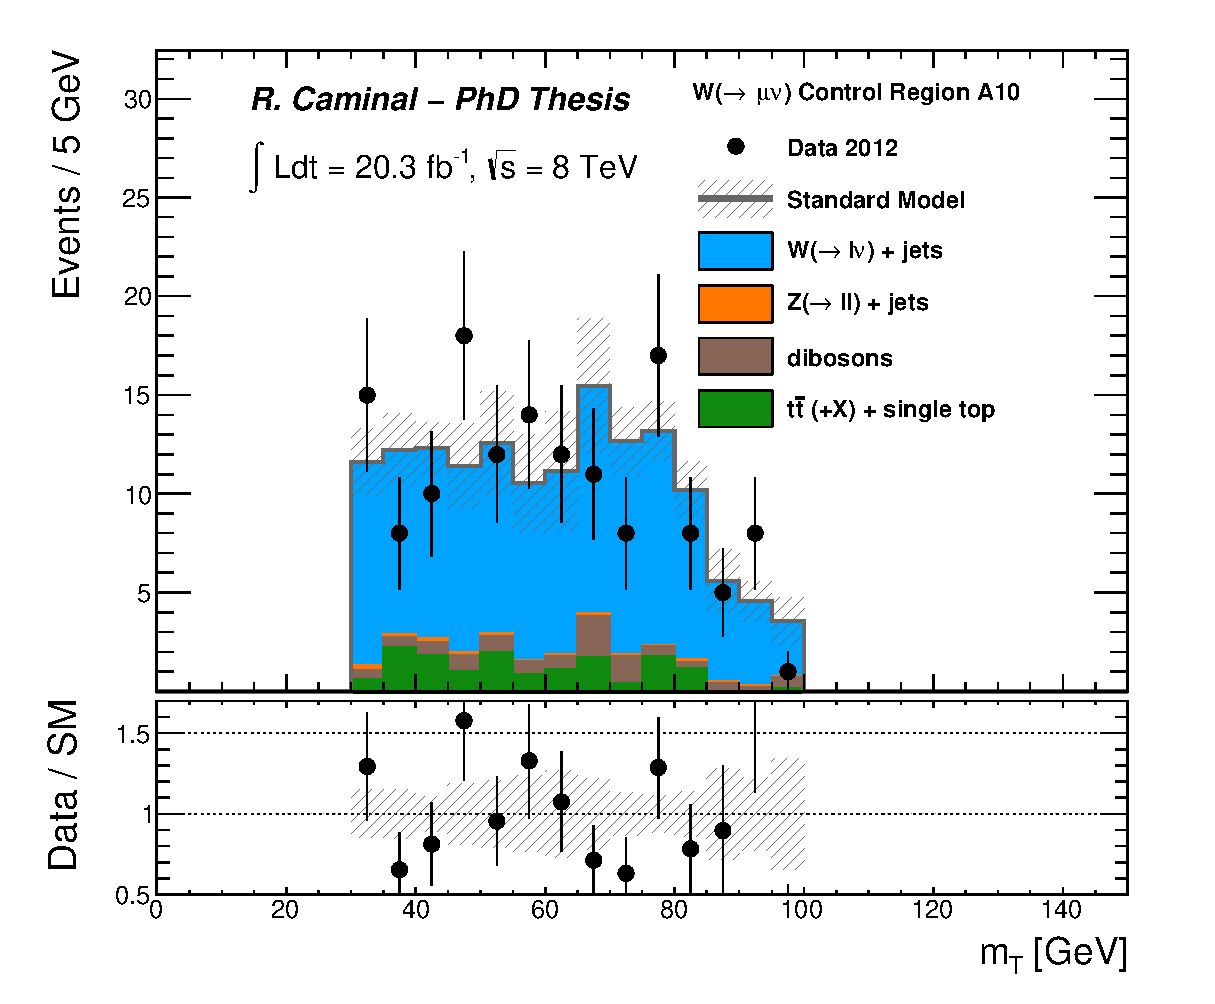
\includegraphics[width=0.495\textwidth]{Appendix_FluctuationM6/Figures/plot_Stop_A10_CRwmn_m_MT_fitted.eps}
    }
  \end{center}
  \caption[Kinematic distributions of the identified muons in the $\wmn$+jets control region for the selection cuts of region M6, after the normalization factors extracted from the fit have been applied.]{The measured kinematic distributions of the identified muons in the $\wmn$+jets control region for the selection cuts of region M6 compared to the background predictions. The latter include the global normalization factors extracted from the fit. The error bands in the ratios include the statistical and experimental uncertainties on the background predictions.}
  \label{fig:Plot_M6_CRwmn_Leptonkinematics}
\end{figure}


\begin{figure}[!ht]
  \begin{center}
    \mbox{
      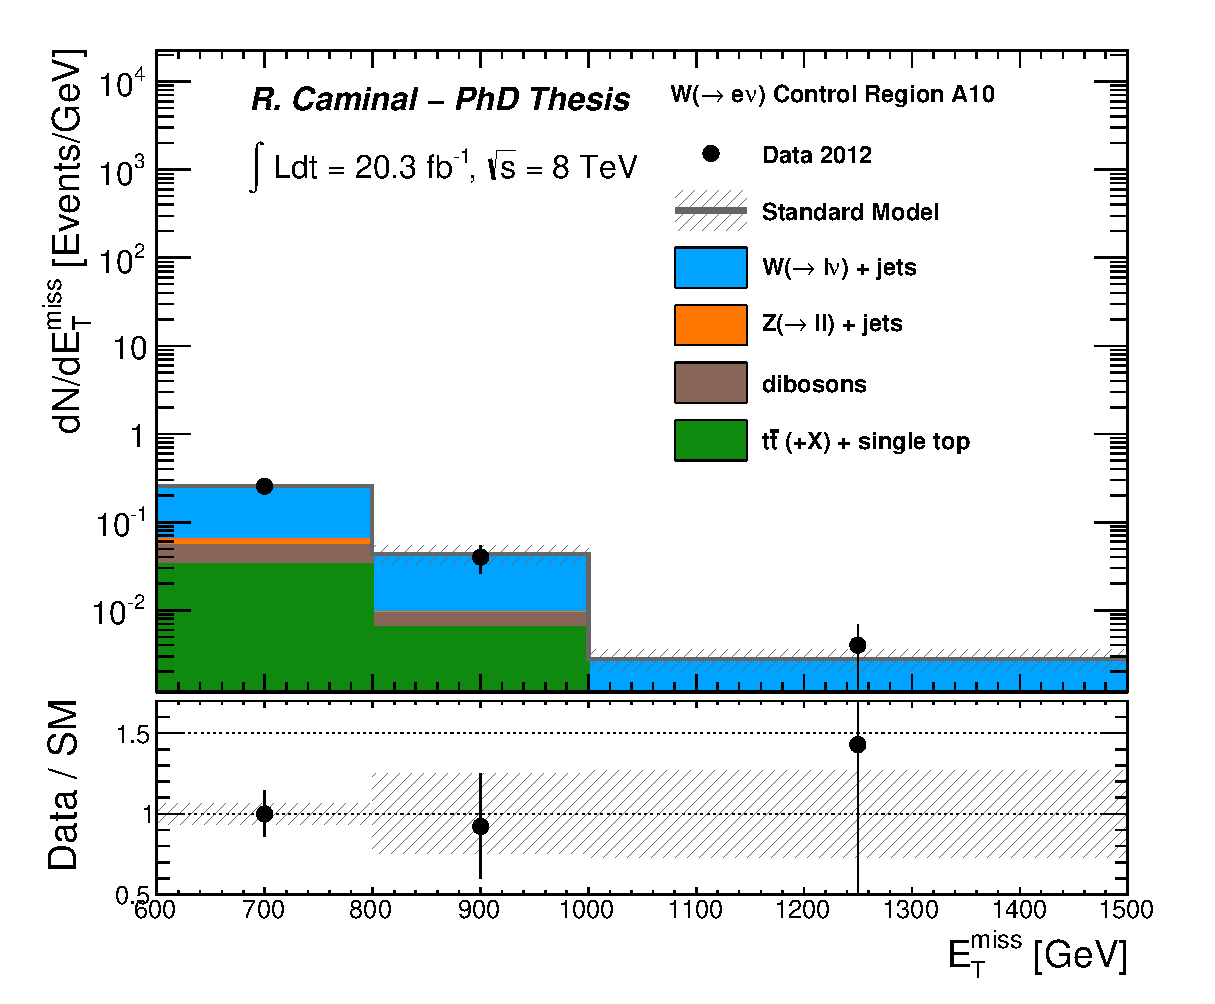
\includegraphics[width=0.495\textwidth]{Appendix_FluctuationM6/Figures/plot_Stop_A10_CRele_met_fitted.eps}
      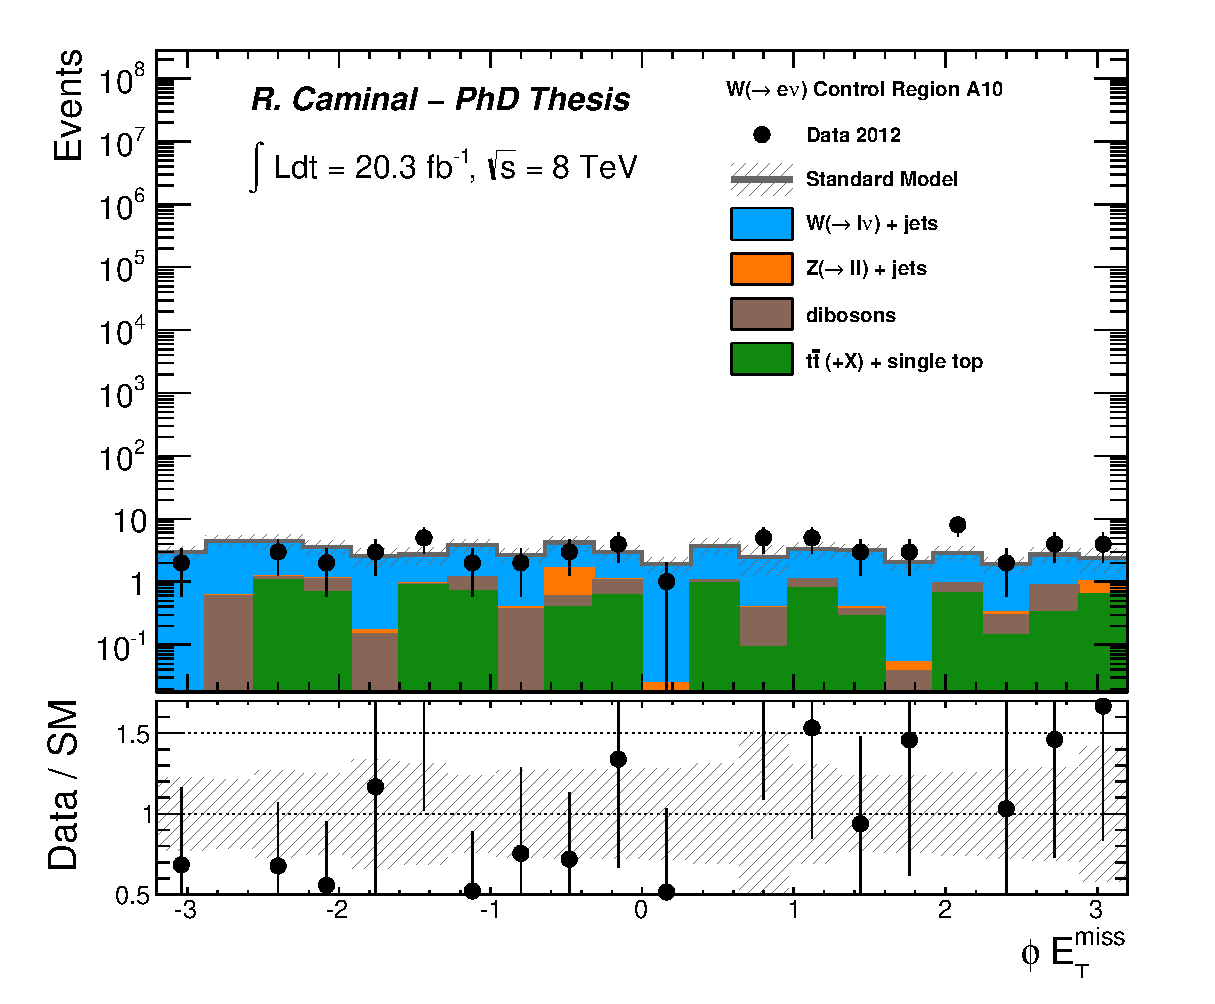
\includegraphics[width=0.495\textwidth]{Appendix_FluctuationM6/Figures/plot_Stop_A10_CRele_met_phi_fitted.eps}
    }
    \mbox{
      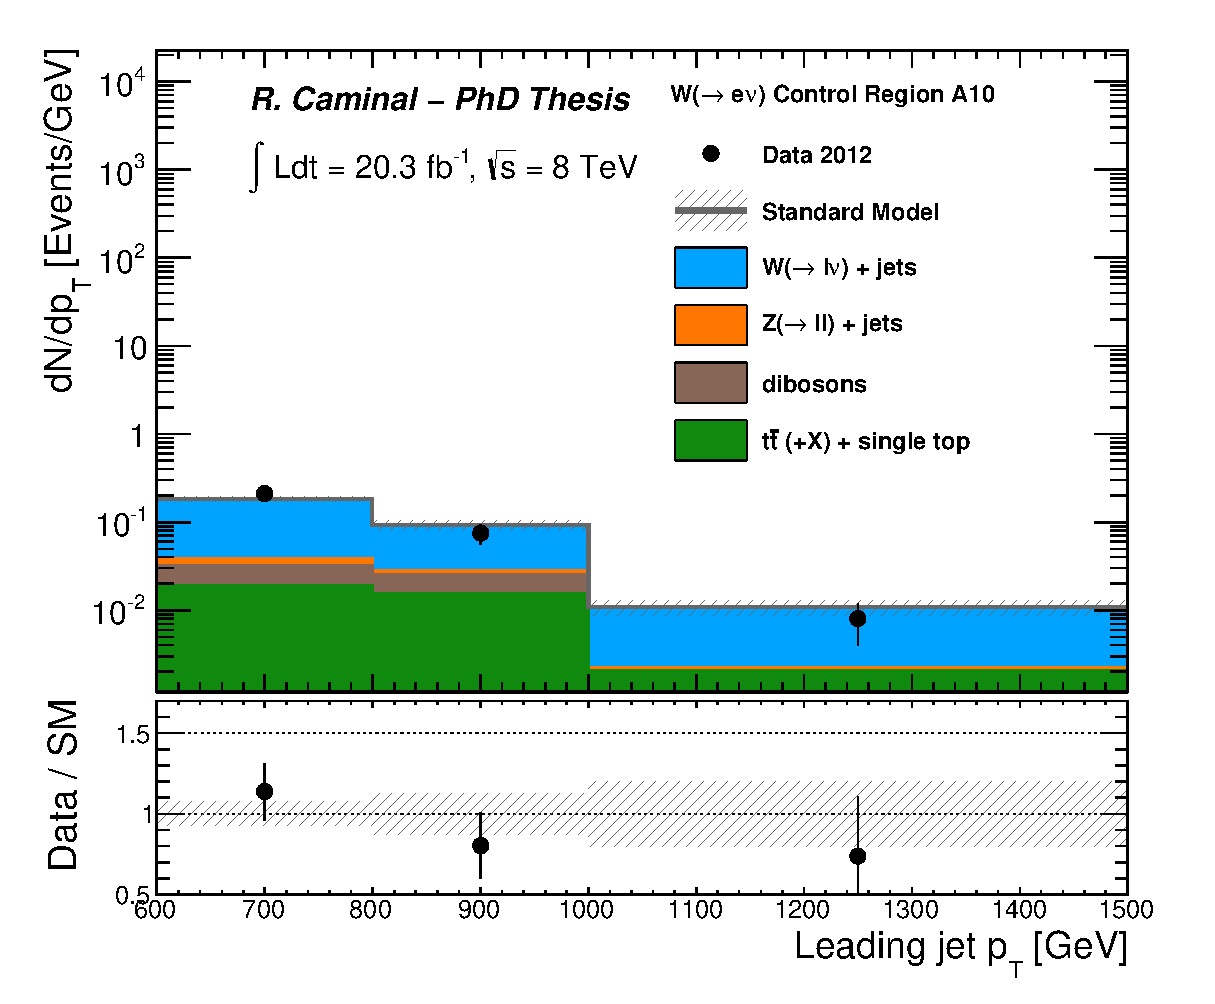
\includegraphics[width=0.495\textwidth]{Appendix_FluctuationM6/Figures/plot_Stop_A10_CRele_pt1_fitted.eps}
      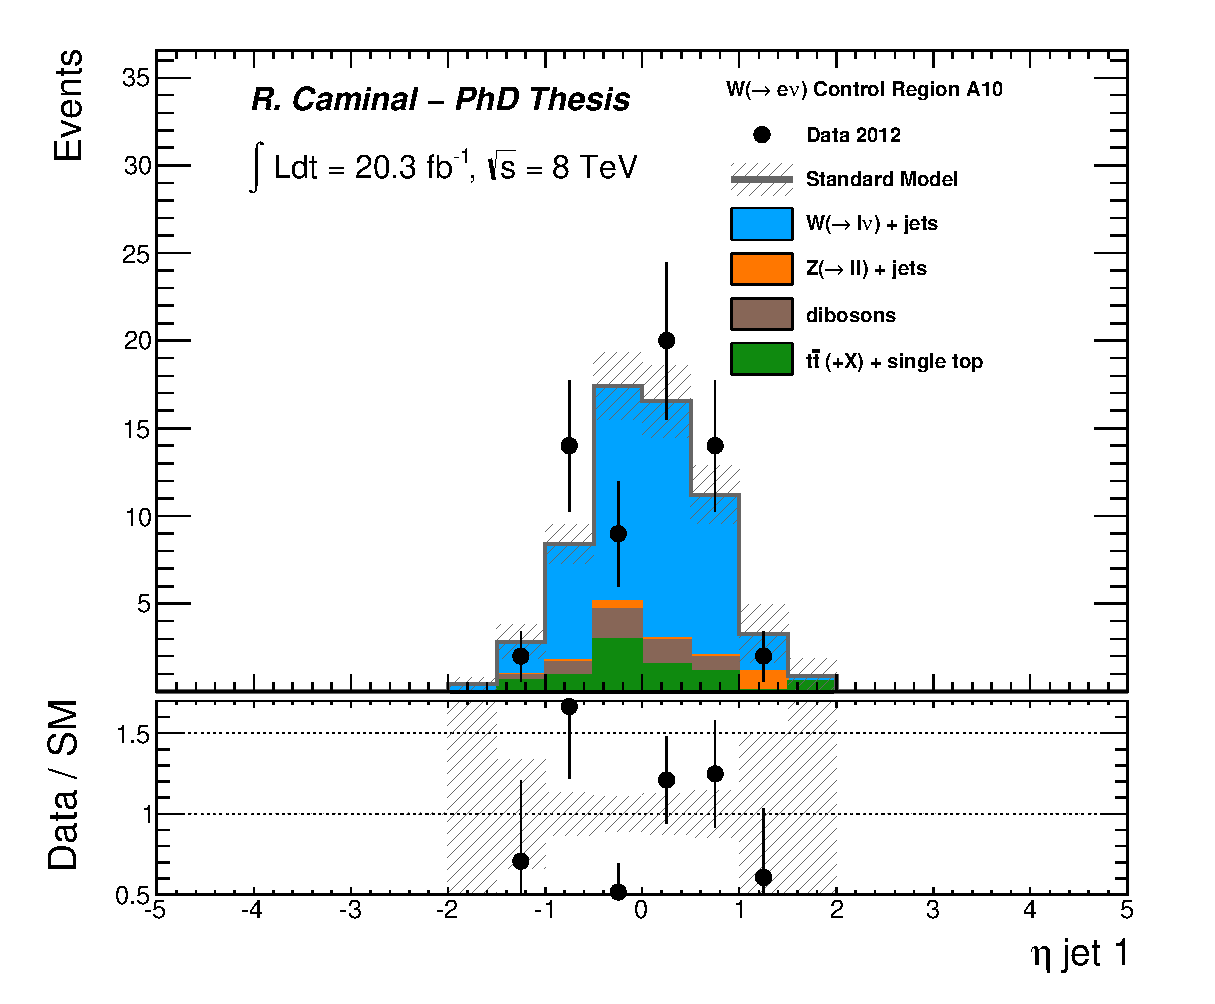
\includegraphics[width=0.495\textwidth]{Appendix_FluctuationM6/Figures/plot_Stop_A10_CRele_eta1_fitted.eps}
    }
    \mbox{
      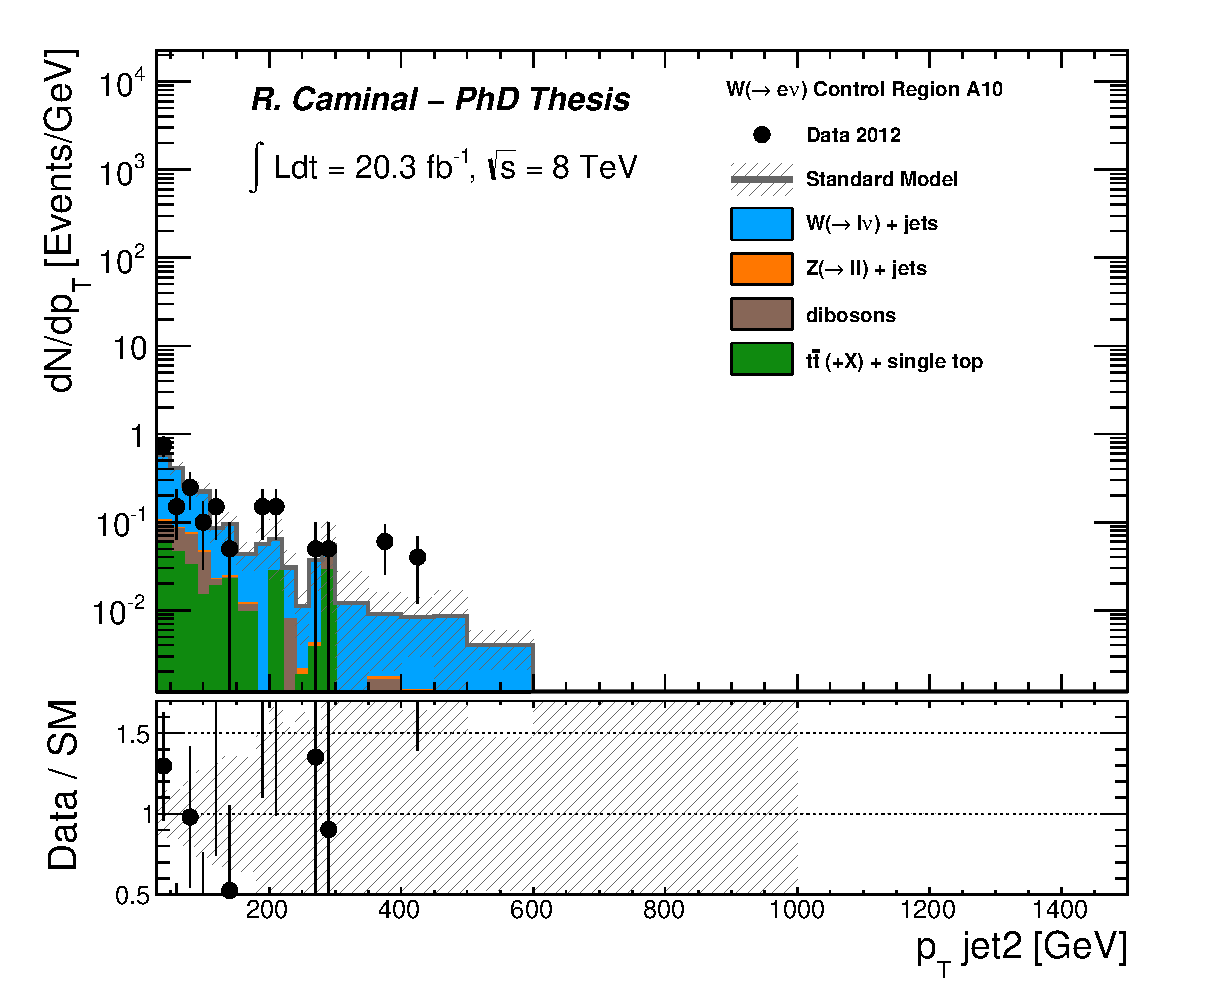
\includegraphics[width=0.495\textwidth]{Appendix_FluctuationM6/Figures/plot_Stop_A10_CRele_pt2_fitted.eps}
      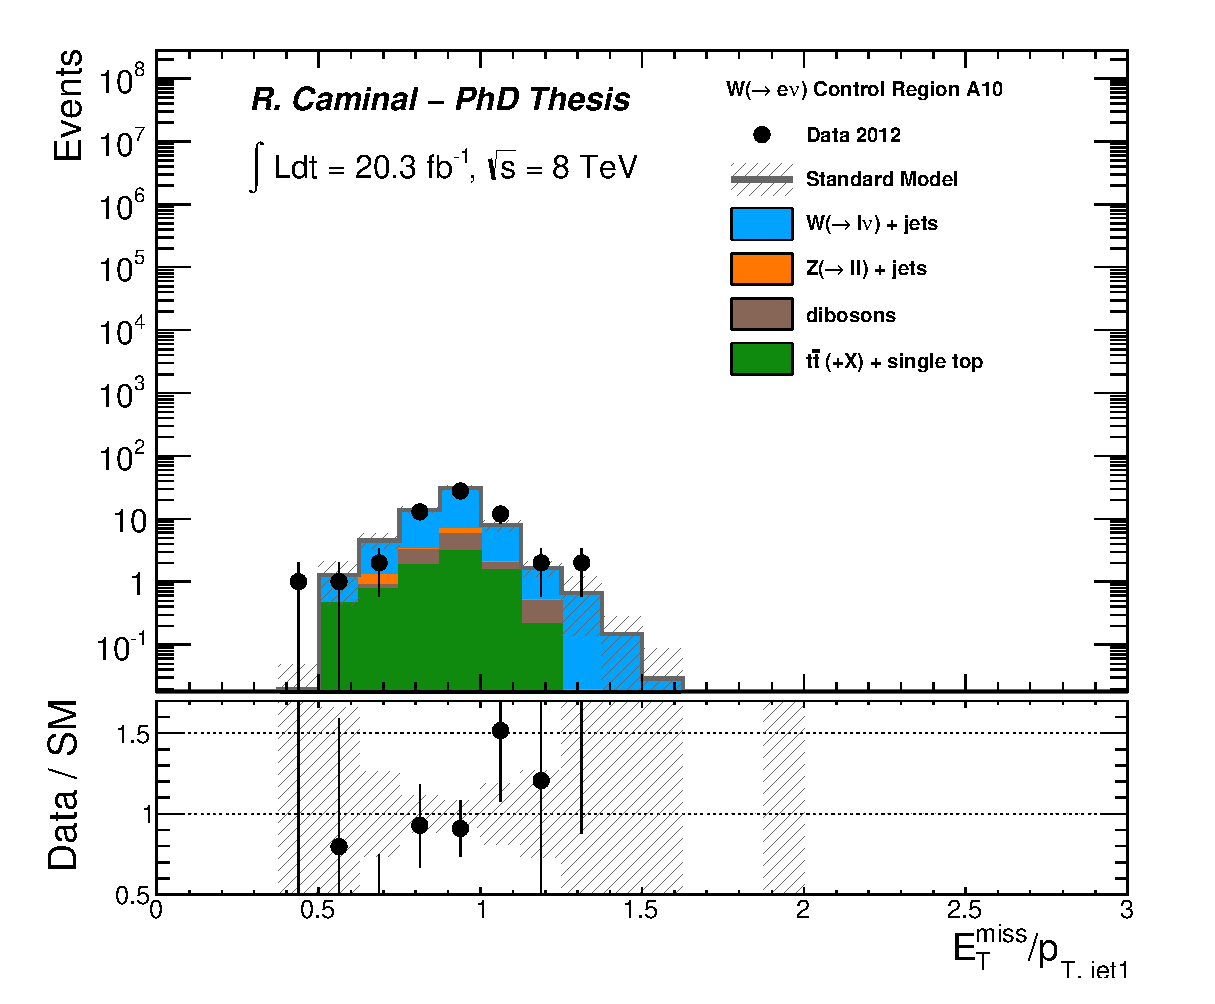
\includegraphics[width=0.495\textwidth]{Appendix_FluctuationM6/Figures/plot_Stop_A10_CRele_metpt1_fitted.eps}
    }
  \end{center}
  \caption[Kinematic distributions of the reconstructed jets and $\met$ in the $\wen$+jets control region for the selection cuts of region M6, after the normalization factors extracted from the fit have been applied.]{The measured kinematic distributions of the reconstructed jets and $\met$ in the $\wen$+jets control region for the selection cuts of region M6 compared to the background predictions. The latter include the global normalization factors extracted from the fit. The error bands in the ratios include the statistical and experimental uncertainties on the background predictions.}
  \label{fig:Plot_M6_CRele_Jetkinematics}
\end{figure}

\begin{figure}[!ht]
  \begin{center}
    \mbox{
      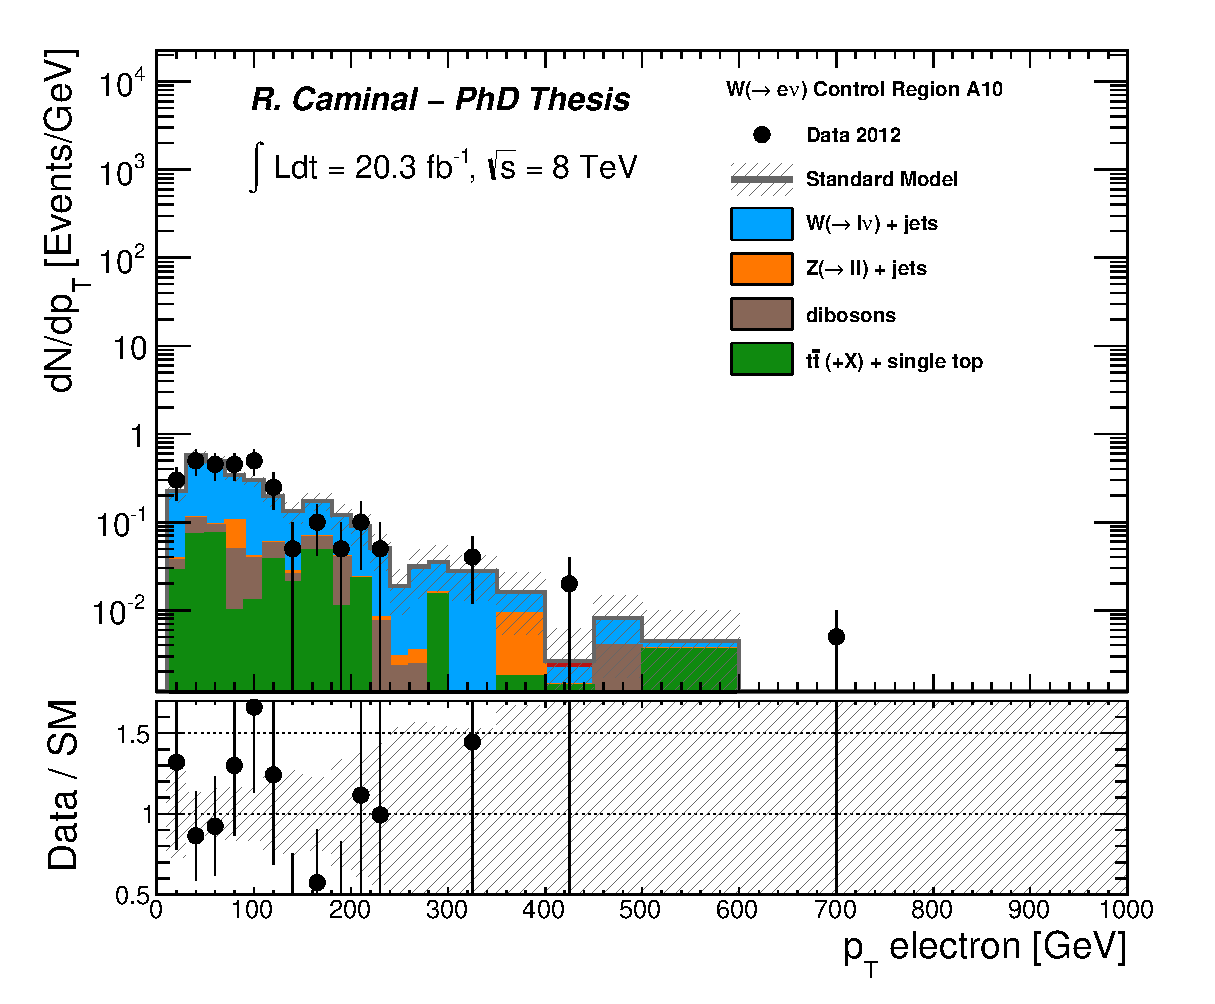
\includegraphics[width=0.495\textwidth]{Appendix_FluctuationM6/Figures/plot_Stop_A10_CRele_e_pt_fitted.eps}
      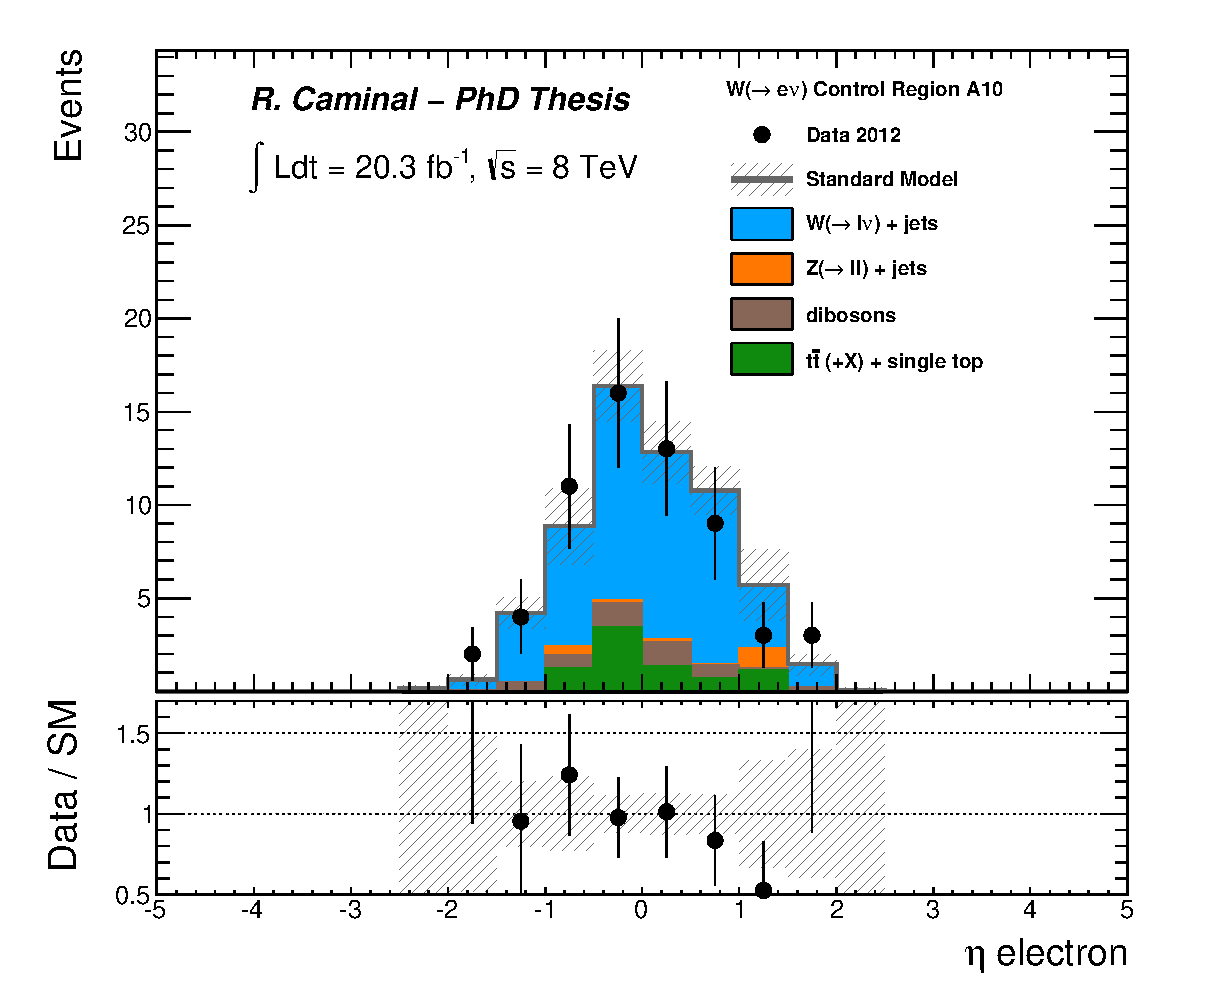
\includegraphics[width=0.495\textwidth]{Appendix_FluctuationM6/Figures/plot_Stop_A10_CRele_e_eta_fitted.eps}
    }
    \mbox{
      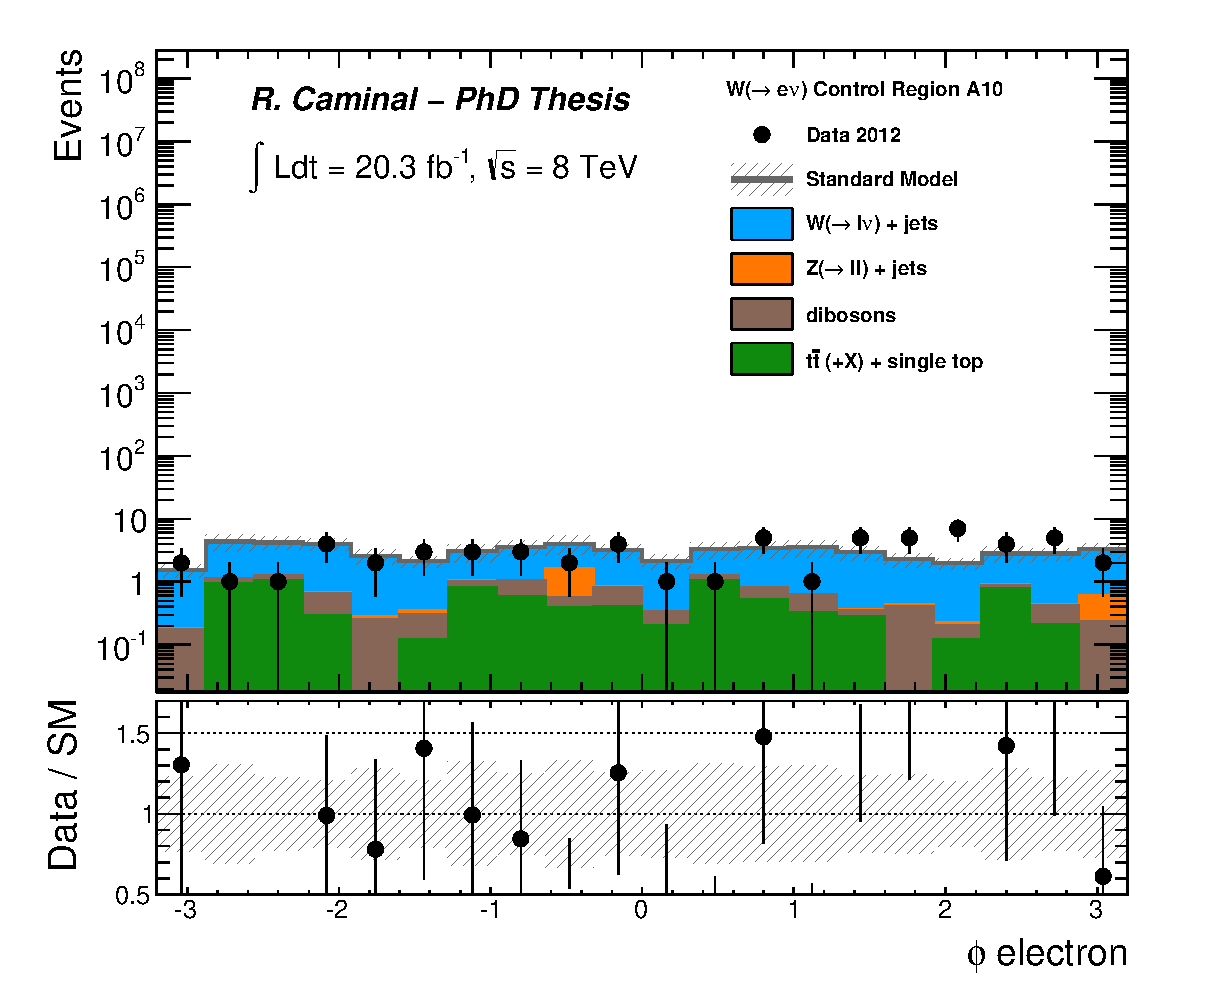
\includegraphics[width=0.495\textwidth]{Appendix_FluctuationM6/Figures/plot_Stop_A10_CRele_e_phi_fitted.eps}
      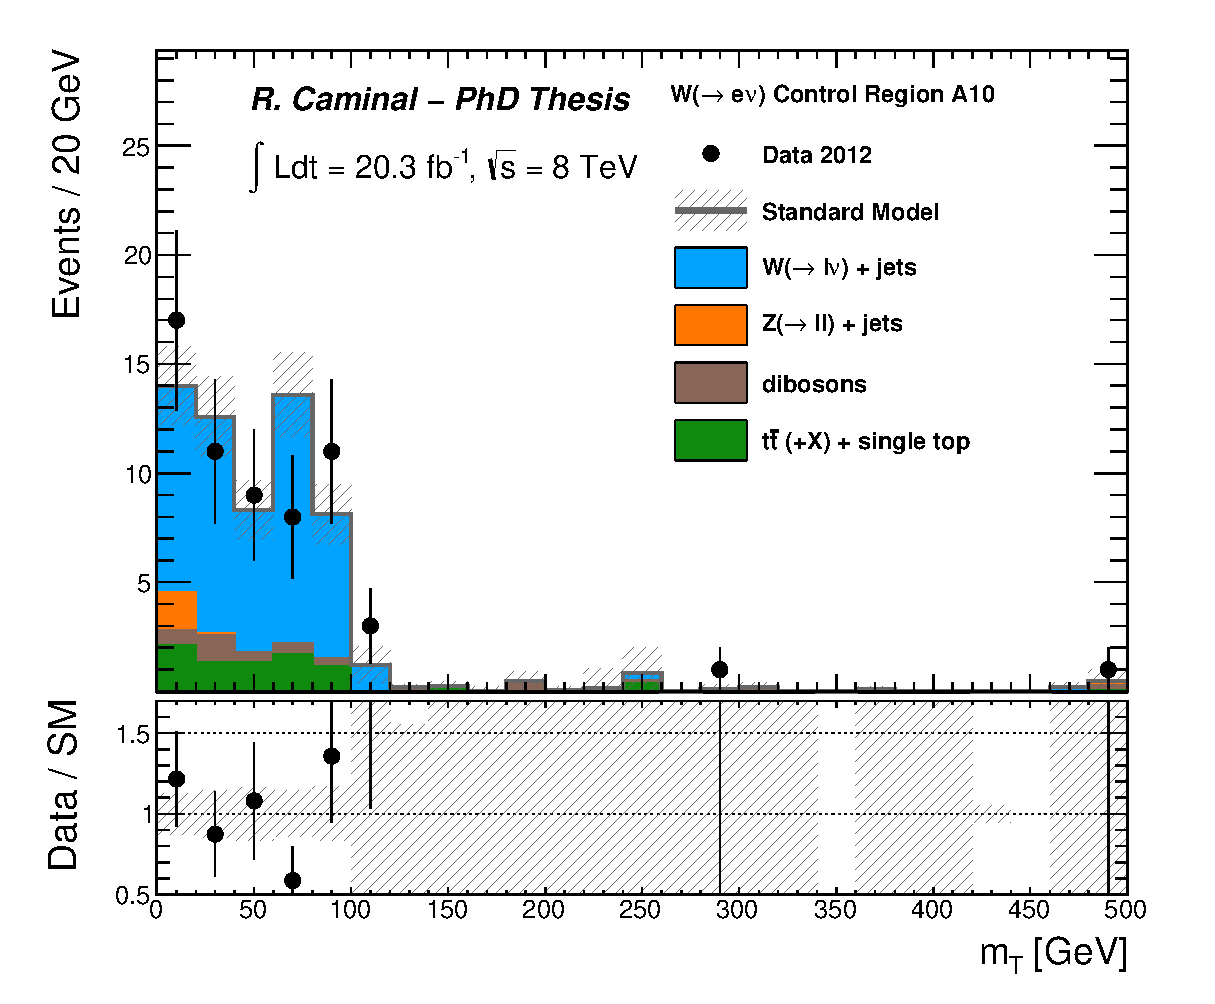
\includegraphics[width=0.495\textwidth]{Appendix_FluctuationM6/Figures/plot_Stop_A10_CRele_e_MT_fitted.eps}
    }
  \end{center}
  \caption[Kinematic distributions of the identified electrons in the $\wen$+jets control region for the selection cuts of region M6, after the normalization factors extracted from the fit have been applied.]{The measured kinematic distributions of the identified electrons in the $\wen$+jets control region for the selection cuts of region M6 compared to the background predictions. The latter include the global normalization factors extracted from the fit. The error bands in the ratios include the statistical and experimental uncertainties on the background predictions.}
  \label{fig:Plot_M6_CRele_Leptonkinematics}
\end{figure}


\begin{figure}[!ht]
  \begin{center}
    \mbox{
      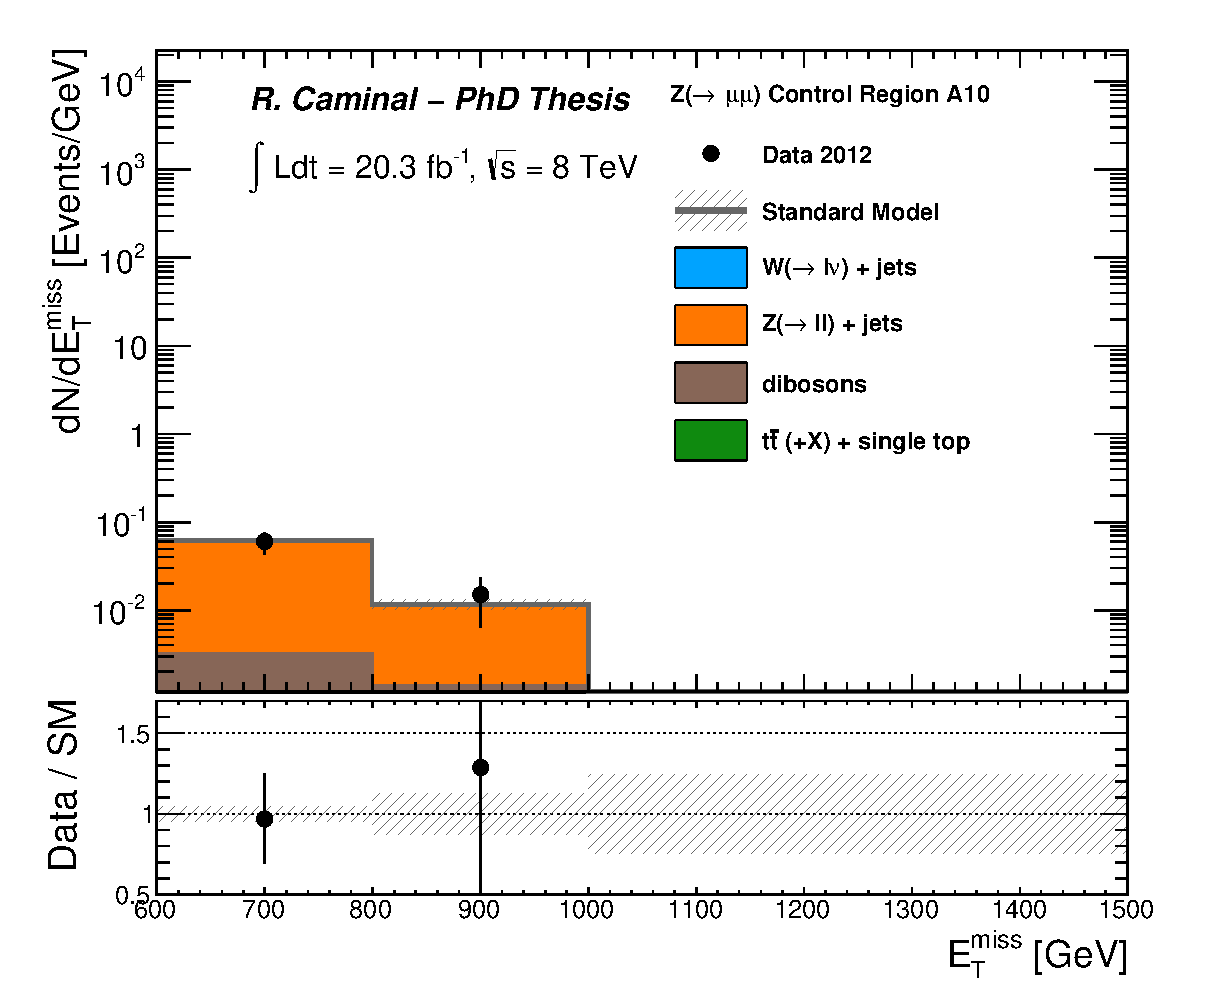
\includegraphics[width=0.495\textwidth]{Appendix_FluctuationM6/Figures/plot_Stop_A10_CRzmm_met_fitted.eps}
      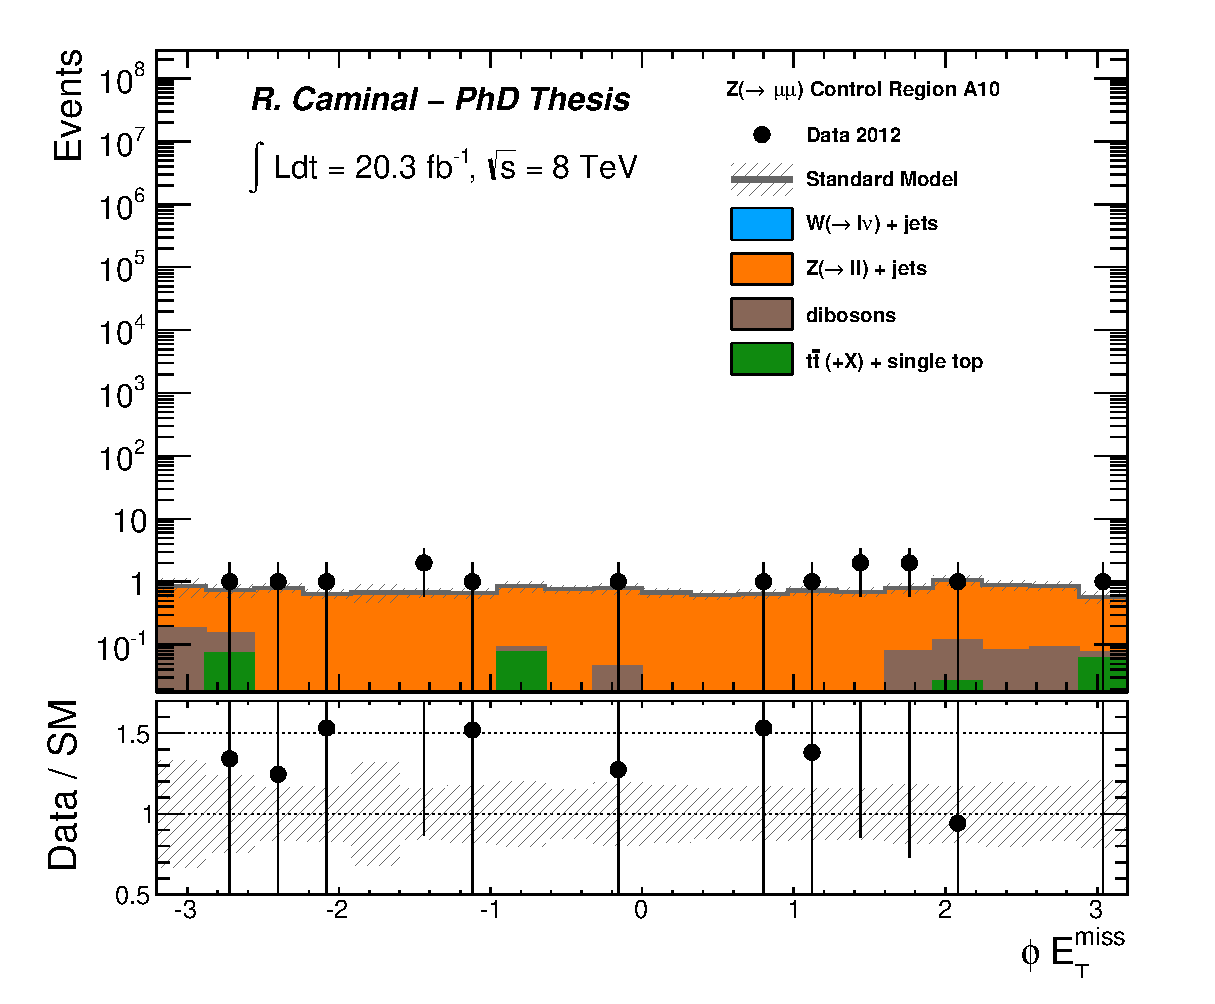
\includegraphics[width=0.495\textwidth]{Appendix_FluctuationM6/Figures/plot_Stop_A10_CRzmm_met_phi_fitted.eps}
    }
    \mbox{
      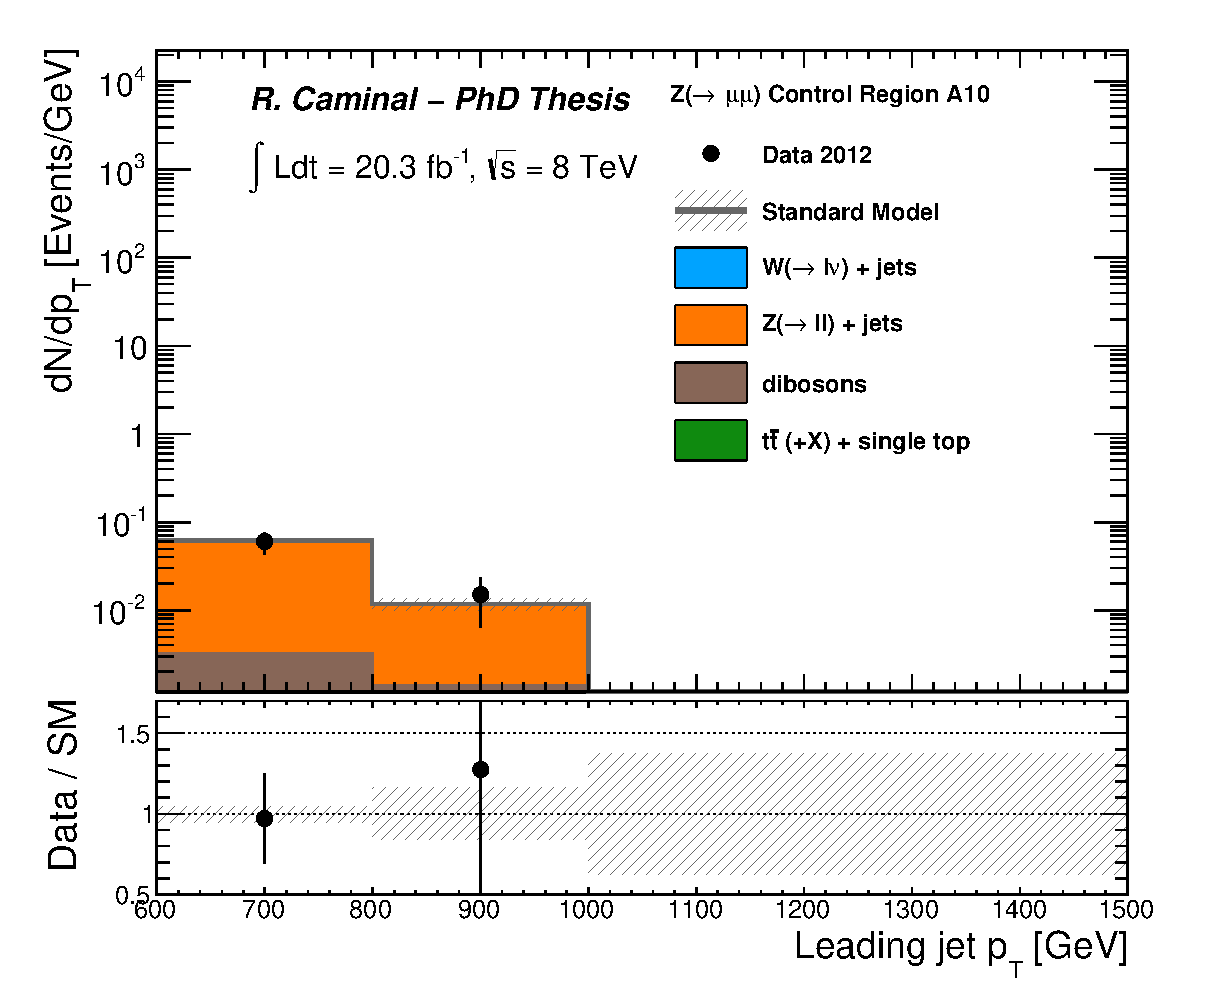
\includegraphics[width=0.495\textwidth]{Appendix_FluctuationM6/Figures/plot_Stop_A10_CRzmm_pt1_fitted.eps}
      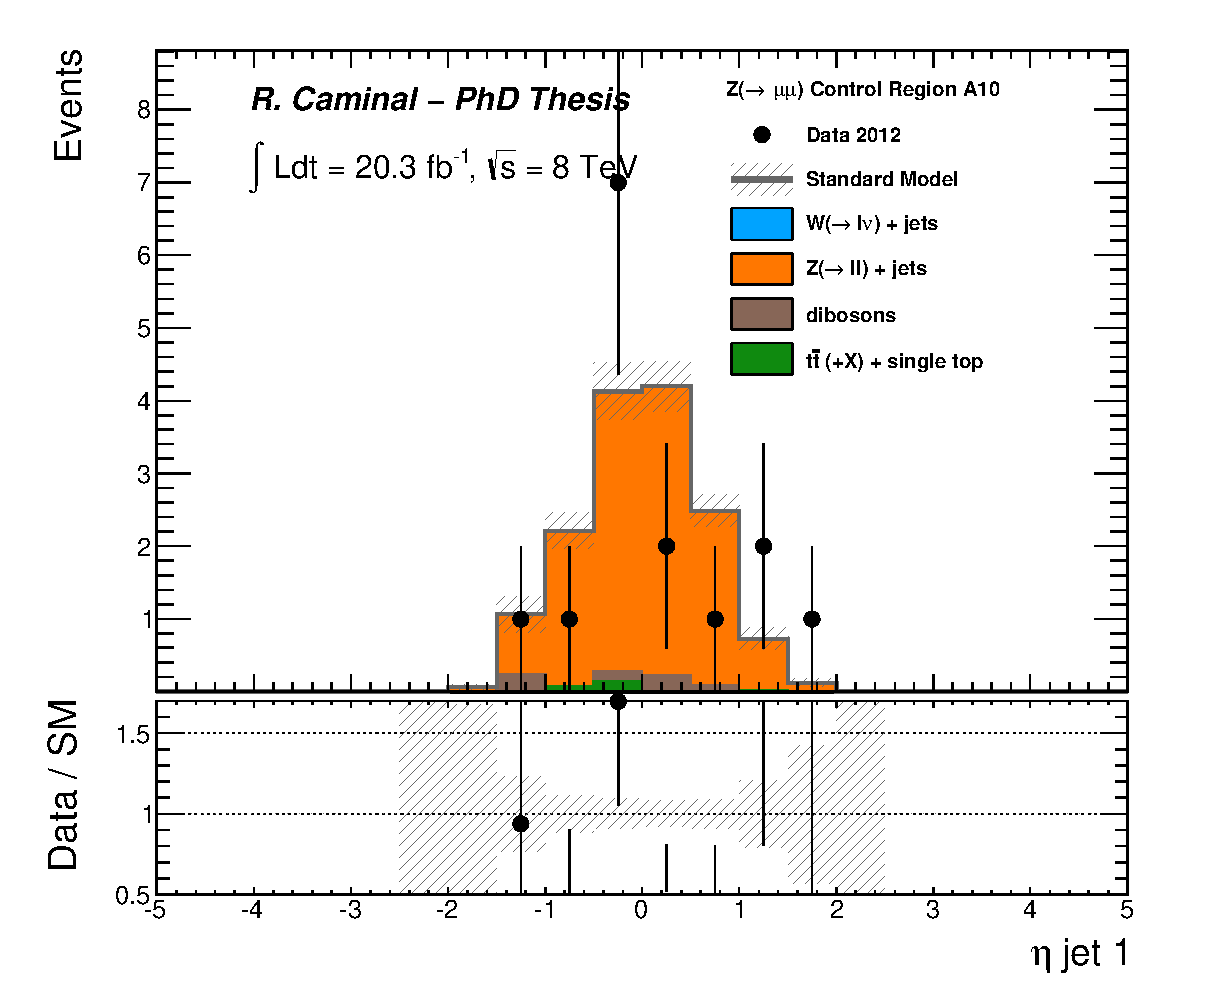
\includegraphics[width=0.495\textwidth]{Appendix_FluctuationM6/Figures/plot_Stop_A10_CRzmm_eta1_fitted.eps}
    }
    \mbox{
      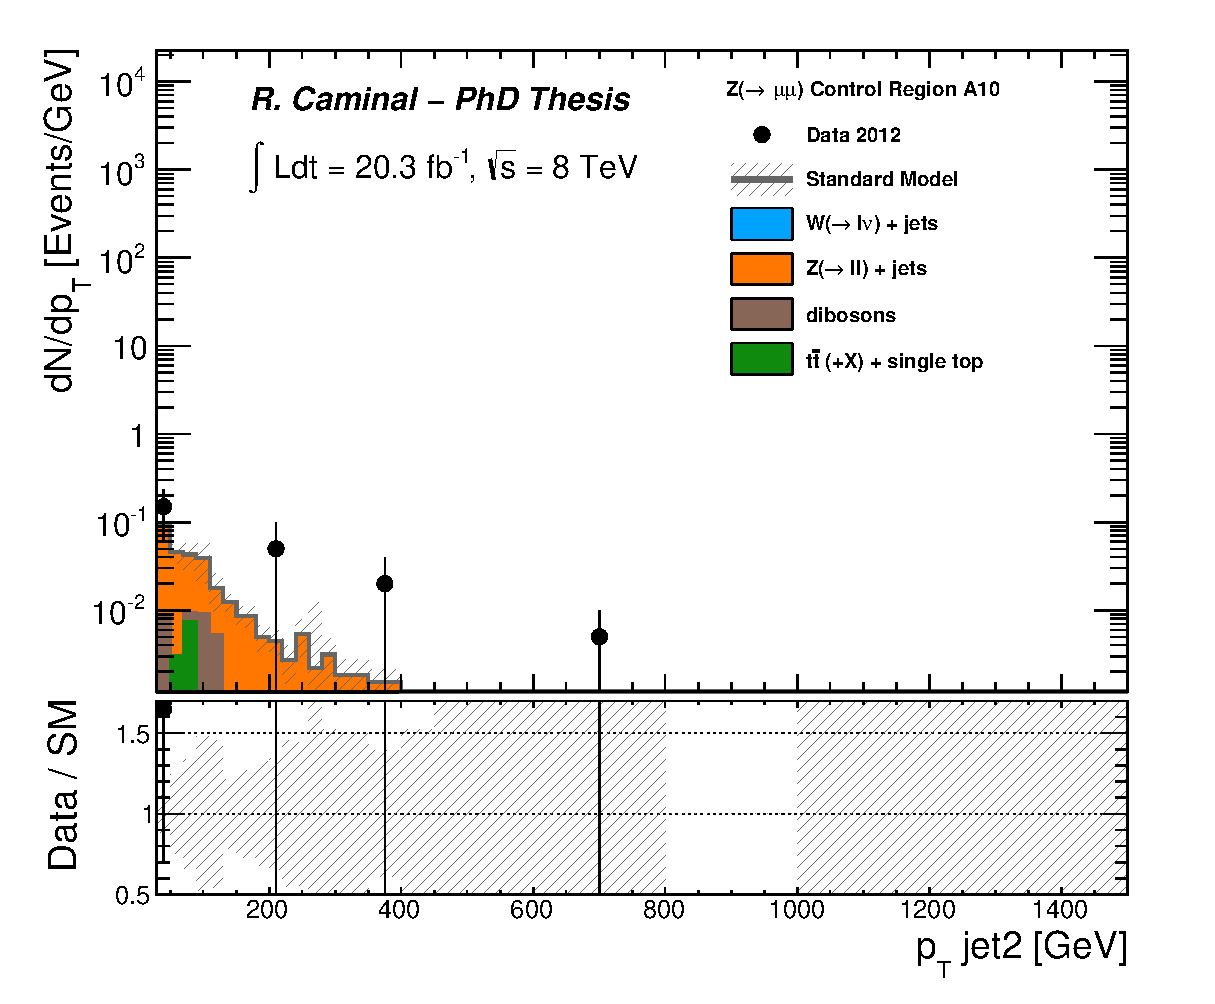
\includegraphics[width=0.495\textwidth]{Appendix_FluctuationM6/Figures/plot_Stop_A10_CRzmm_pt2_fitted.eps}
      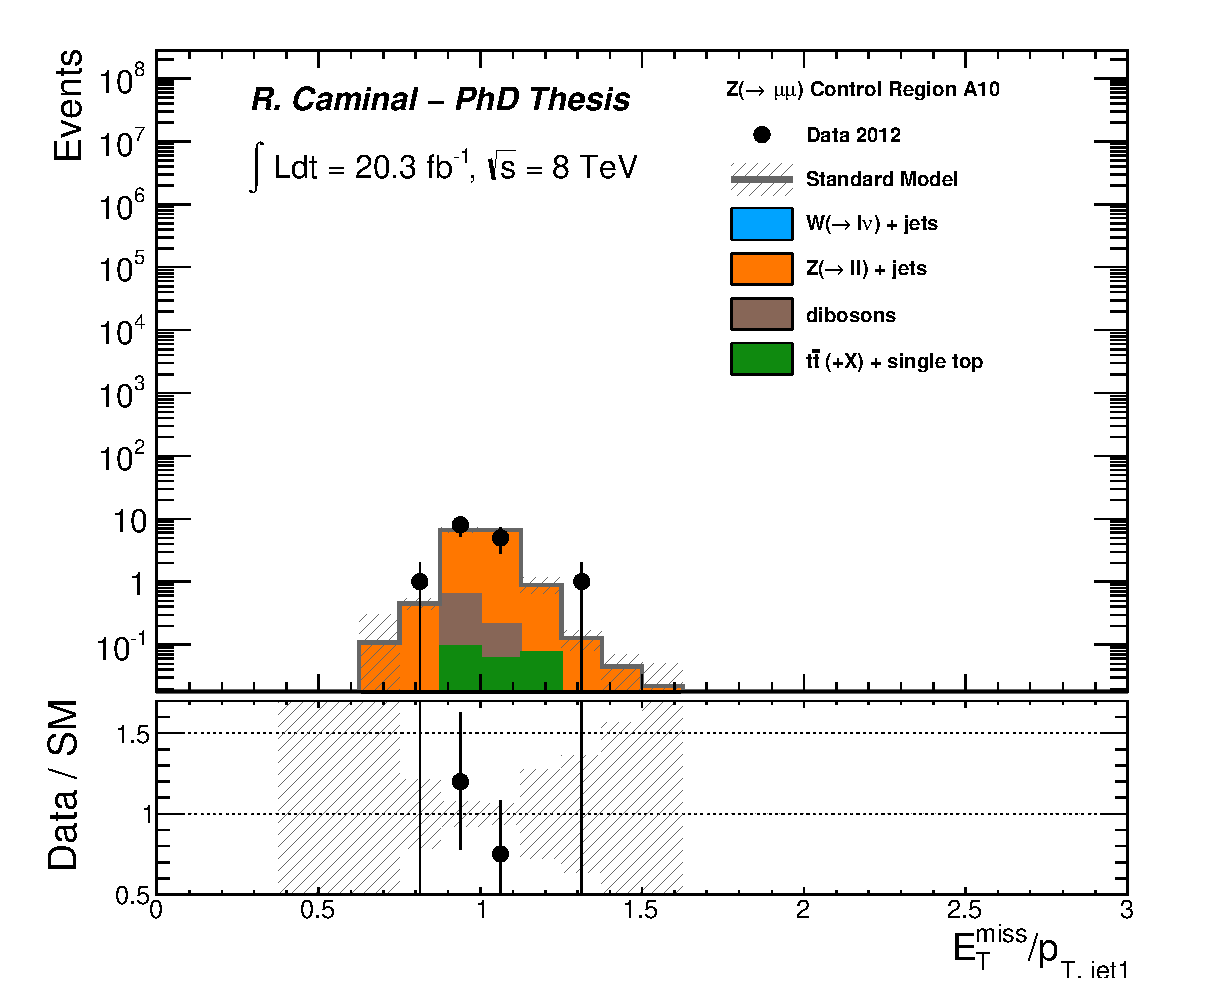
\includegraphics[width=0.495\textwidth]{Appendix_FluctuationM6/Figures/plot_Stop_A10_CRzmm_metpt1_fitted.eps}
    }
  \end{center}
  \caption[Kinematic distributions of the reconstructed jets and $\met$ in the $\zmm$+jets control region for the selection cuts of region M6, after the normalization factors extracted from the fit have been applied.]{The measured kinematic distributions of the reconstructed jets and $\met$ in the $\zmm$+jets control region for the selection cuts of region M6 compared to the background predictions. The latter include the global normalization factors extracted from the fit. The error bands in the ratios include the statistical and experimental uncertainties on the background predictions.}
  \label{fig:Plot_M6_CRzmm_Jetkinematics}
\end{figure}

\begin{figure}[!ht]
  \begin{center}
    \mbox{
      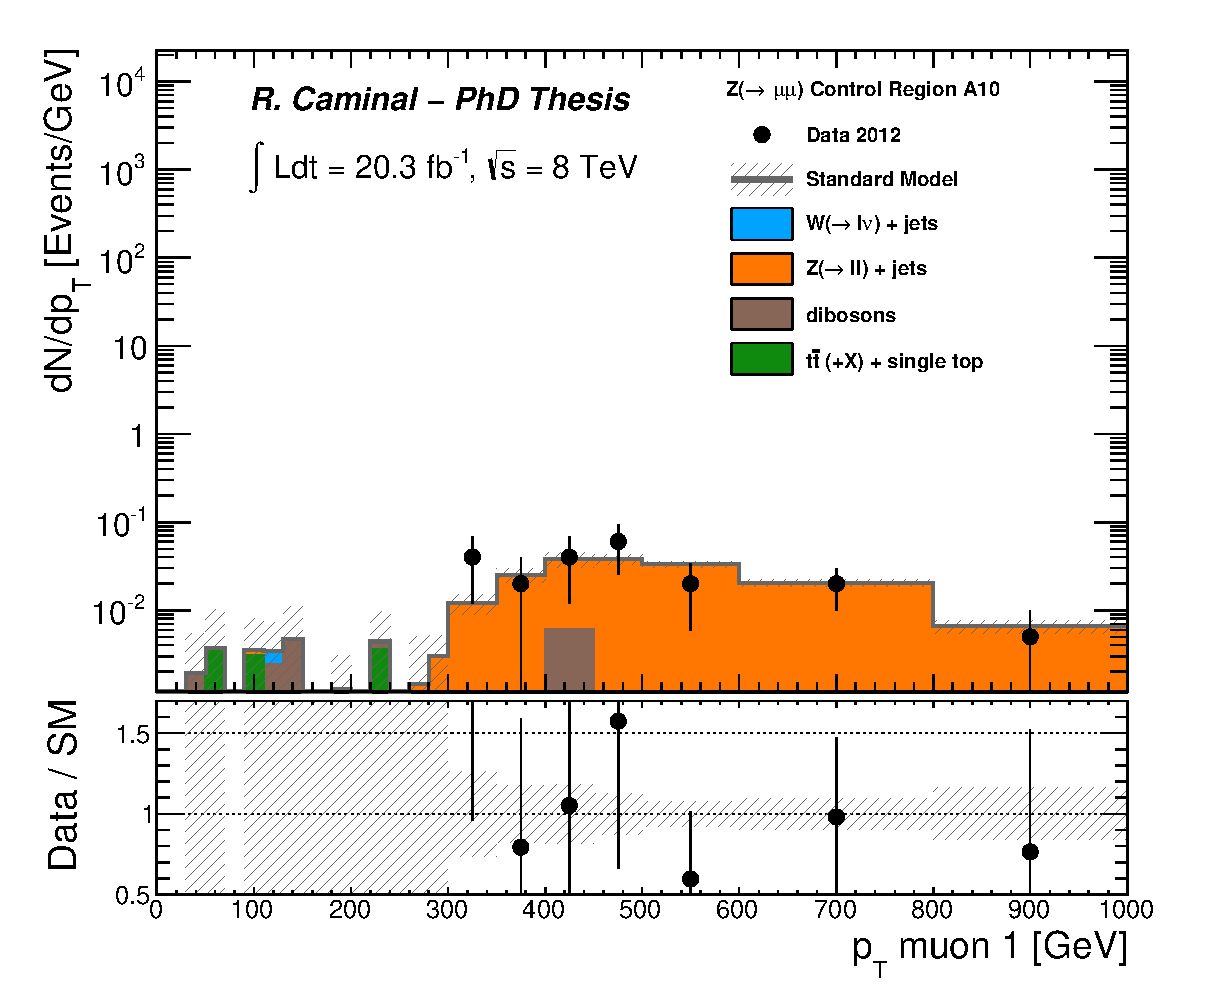
\includegraphics[width=0.495\textwidth]{Appendix_FluctuationM6/Figures/plot_Stop_A10_CRzmm_m_pt_fitted.eps}
      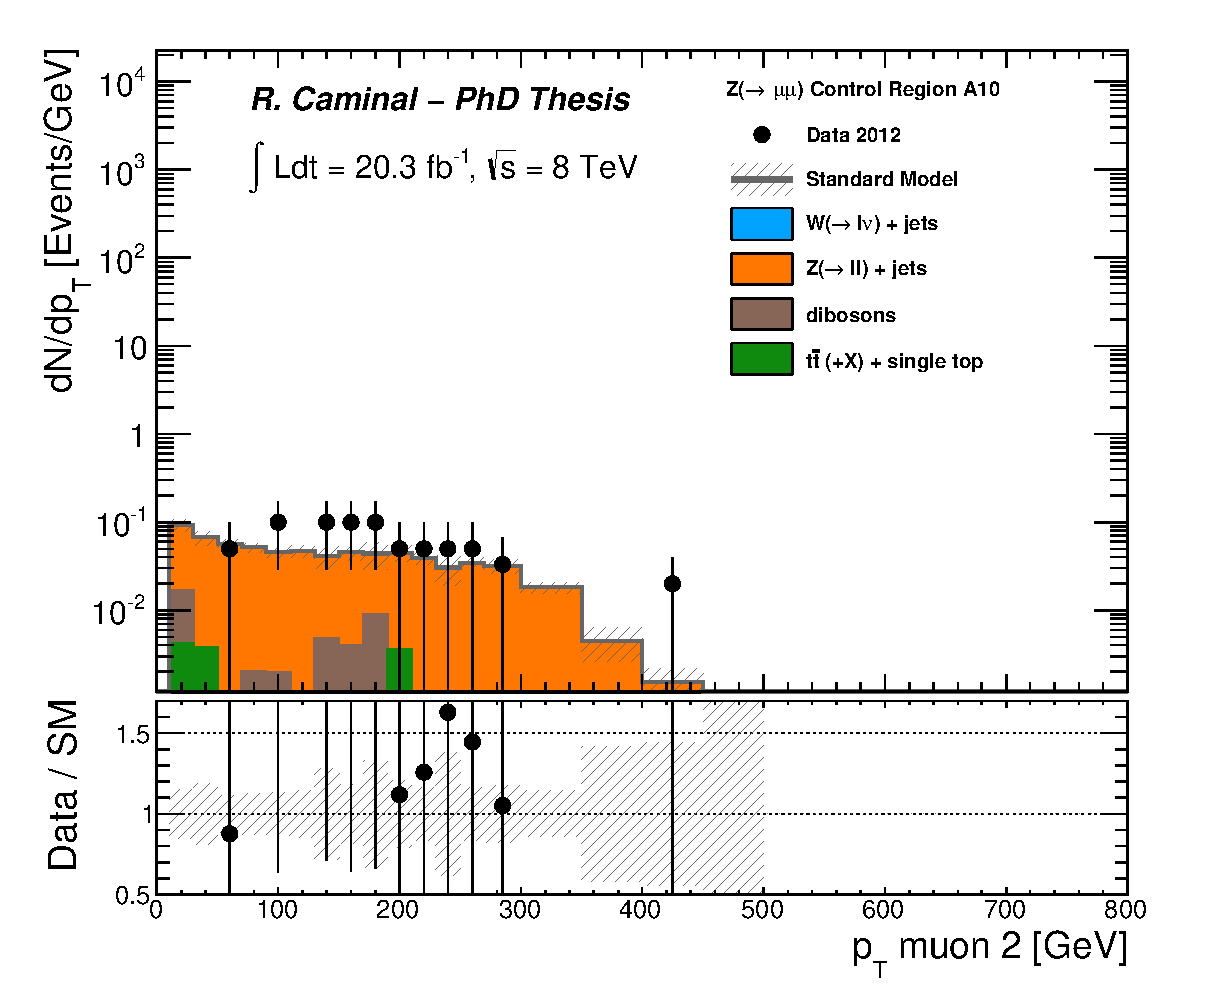
\includegraphics[width=0.495\textwidth]{Appendix_FluctuationM6/Figures/plot_Stop_A10_CRzmm_m2_pt_fitted.eps}
    }
    \mbox{
      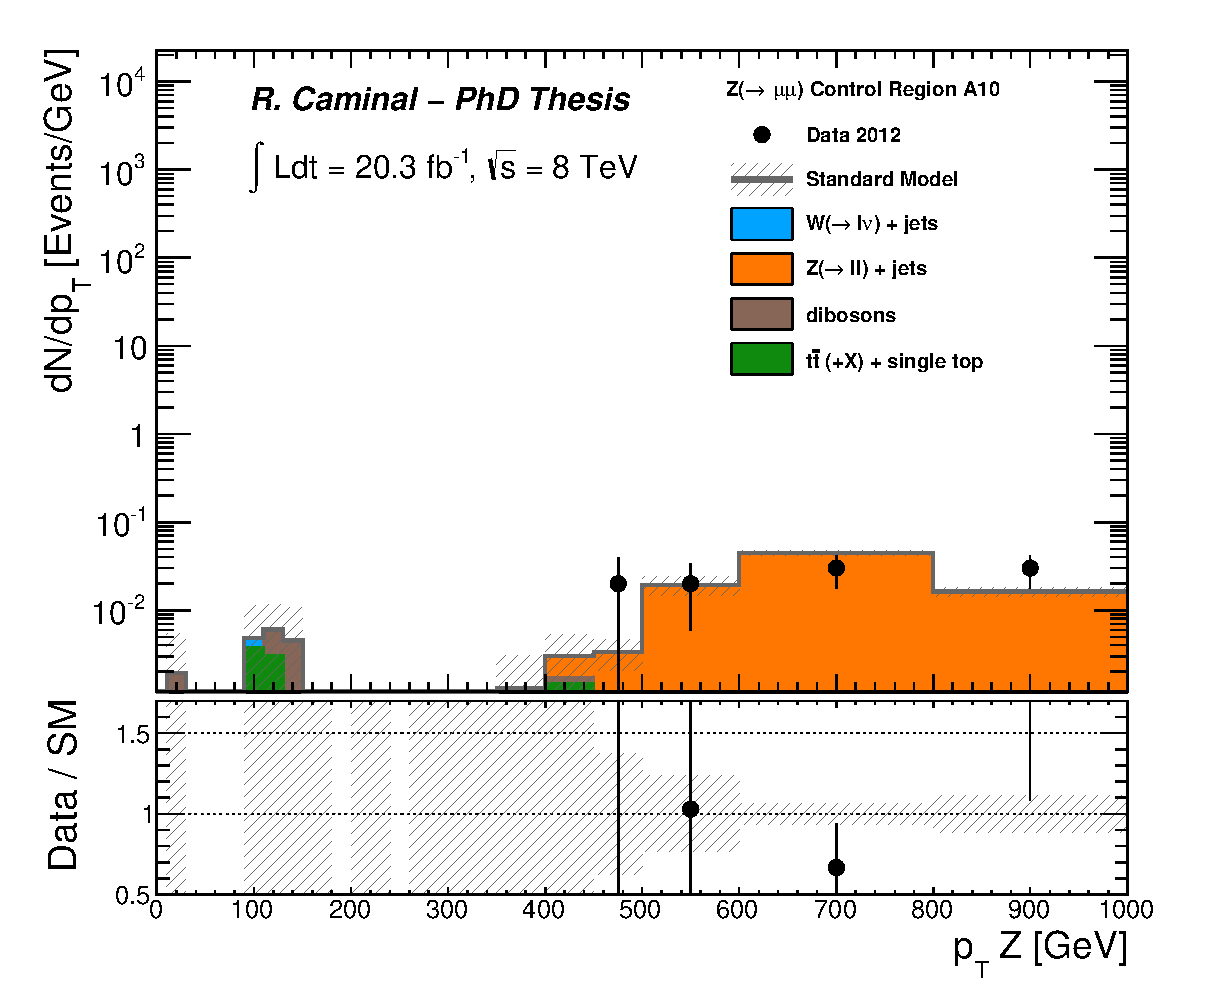
\includegraphics[width=0.495\textwidth]{Appendix_FluctuationM6/Figures/plot_Stop_A10_CRzmm_m_Zpt_fitted.eps}
      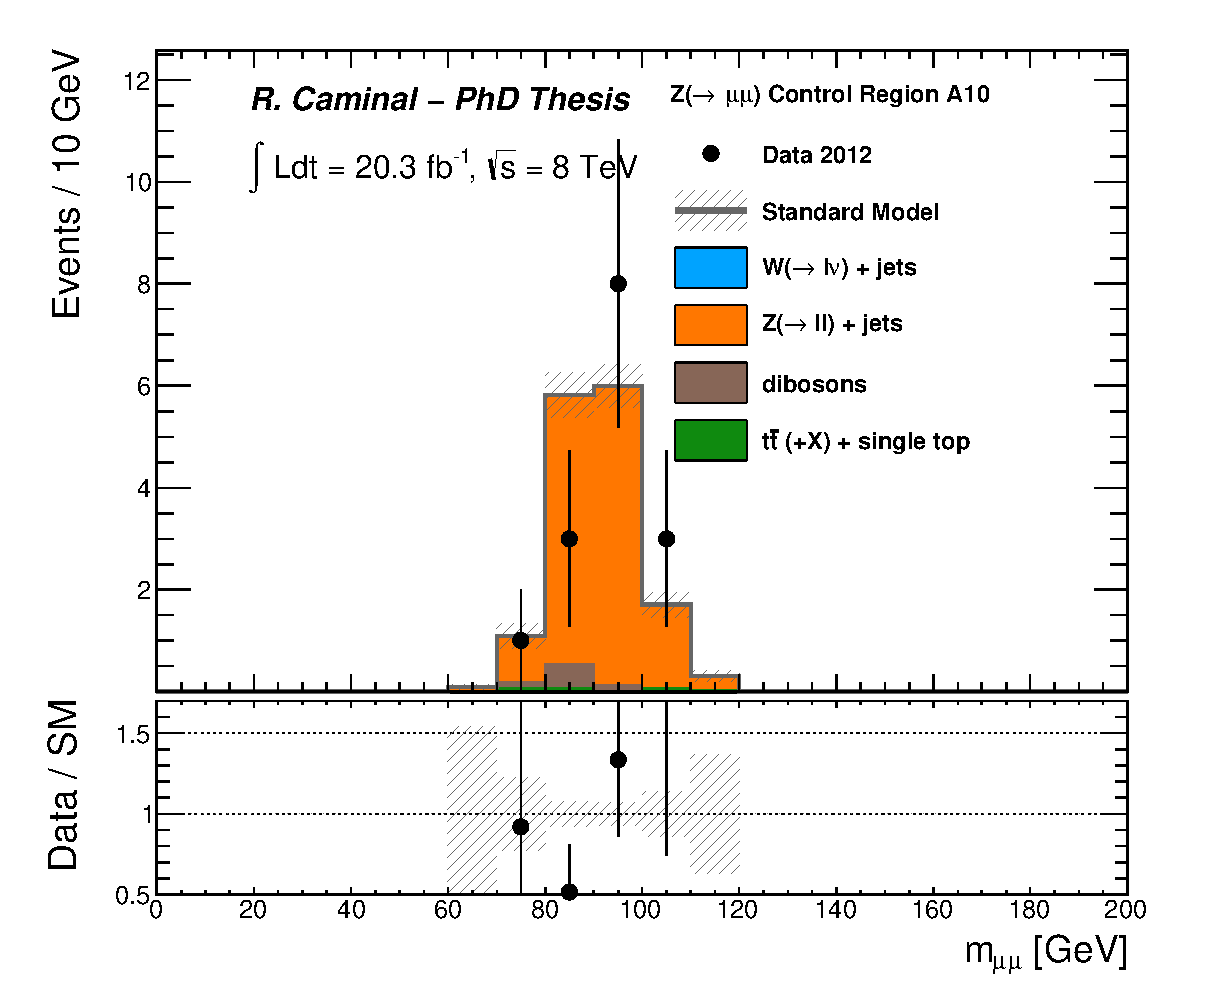
\includegraphics[width=0.495\textwidth]{Appendix_FluctuationM6/Figures/plot_Stop_A10_CRzmm_m_M_fitted.eps}
    }
  \end{center}
  \caption[Kinematic distributions of the identified muons in the $Z/\gamma^{\ast}(\rightarrow \mu^{+}\mu^{-})$+jets control region for the selection cuts of region M6, after the normalization factors extracted from the fit have been applied.]{The measured kinematic distributions of the identified muons in the $\zmm$ control region for the selection cuts of region M6 compared to the background predictions. The latter include the global normalization factors extracted from the fit. The error bands in the ratios include the statistical and experimental uncertainties on the background predictions.}
  \label{fig:Plot_M6_CRzmm_Leptonkinematics}
\end{figure}

After a careful check of the distributions for the different variables in the control regions, no mismodeling has been observed.
The distributions in the signal region (Figures~\ref{fig:Plot_M1_SR_met} to \ref{fig:Plot_M1_SR_metpt1}, \ref{fig:Plot_M6_SR_Jet1} and \ref{fig:Plot_M6_SR_Jet2}) lead to the same conclusions.

Table~\ref{tab:scaleFactors} points to a downwards fluctuation in the normalization factor \texttt{mu\_Ele}, with respect to M5.
This is the factor used to normalize $\wtn$, the second largest background in the monojet analysis.
Figure~\ref{fig:FluctuationM6scaleFactors} shows the normalization factors \texttt{mu\_Ele}, \texttt{mu\_Wmn} and \texttt{mu\_Zmm} for different $\met$ and leading jet $\pt$ thresholds.
A light downwards fluctuation in \texttt{mu\_Ele}, consistent within statistical uncertainties, is observed for thresholds around 600~GeV, which corresponds to the definition of the signal region M6.

This study concludes that the downward statistical fluctuation observed in the normalization factor, probably combined to an upwards statistical fluctuation of the data in the signal region M6, is the reason for the two sigma-level excess observed, that only new data can resolve.

\begin{figure}[!ht]
  \begin{center}
    \mbox{
      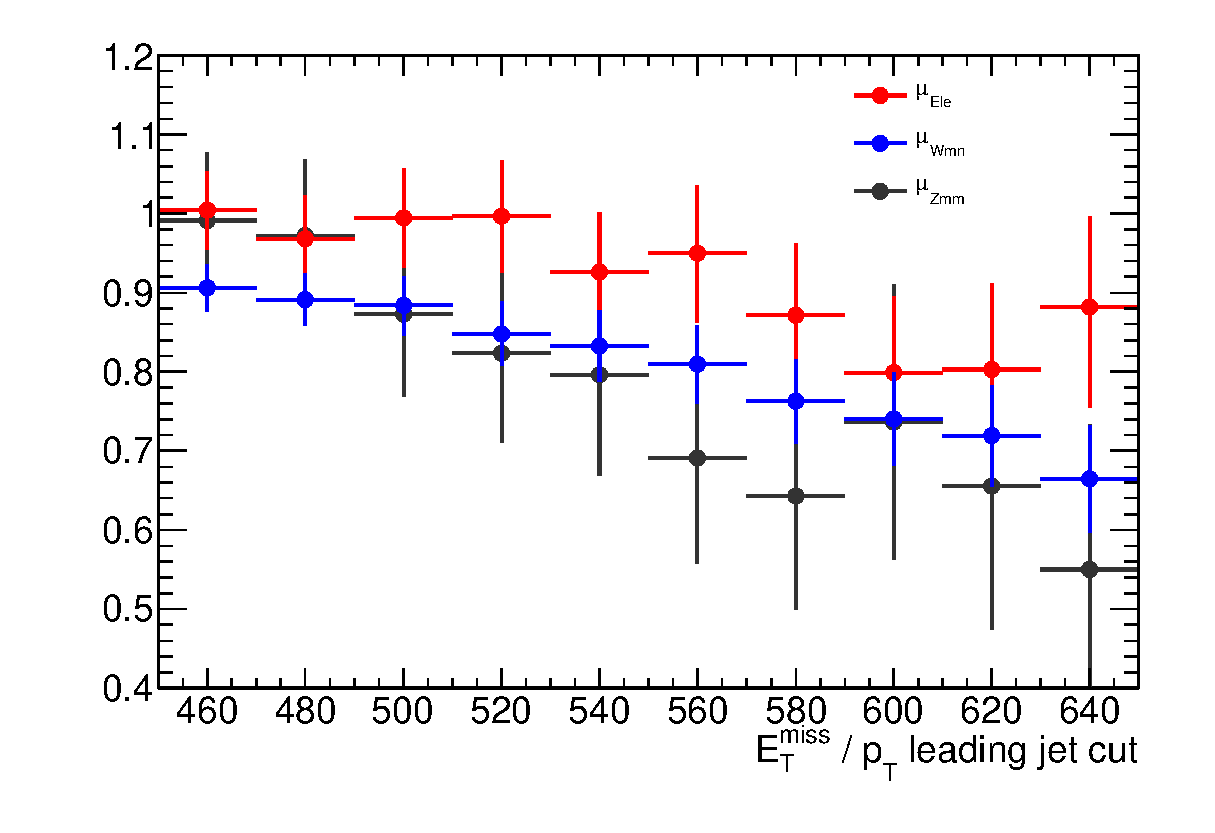
\includegraphics[width=0.995\textwidth]{Appendix_FluctuationM6/Figures/scaleFactorsPlot.eps}
    }
  \end{center}
  \caption{The normalization factors (including only statistical uncertainties on the data) for the monojet selection for different cuts on $\met$ and leading jet $\pt$.}
  \label{fig:FluctuationM6scaleFactors}
\end{figure}

